\documentclass[conference]{IEEEtran}
\IEEEoverridecommandlockouts
\usepackage{cite}
\usepackage{amsmath,amssymb,amsfonts}
\usepackage{algorithmic}
\usepackage{graphicx}
\usepackage{textcomp}
\usepackage{xcolor}
\usepackage{booktabs}
\usepackage{float}
\usepackage{array}
\usepackage{tabularx}
\usepackage{placeins}
\usepackage{url}
\def\BibTeX{{\rm B\kern-.05em{\sc i\kern-.025em b}\kern-.08em
    T\kern-.1667em\lower.7ex\hbox{E}\kern-.125emX}}

\begin{document}
\raggedbottom

\title{Data Cleaning Software for Advanced Driver Assistance Systems (ADAS)}

\author{
\IEEEauthorblockN{Priyanshi}
\IEEEauthorblockA{
\textit{Department of Electronics and} \\
\textit{Electrical Engineering} \\
\textit{MIT World Peace University} \\
Pune, India \\
priyanshi.kochar@mitwpu.edu.in}
\and
\IEEEauthorblockN{Avdhi Kasliwal}
\IEEEauthorblockA{
\textit{Department of Electronics and} \\
\textit{Electrical Engineering} \\
\textit{MIT World Peace University} \\
Pune, India \\
avdhi.kasliwal@mitwpu.edu.in}
\and
\IEEEauthorblockN{Krupa Khandelwal}
\IEEEauthorblockA{
\textit{Department of Electronics and} \\
\textit{Electrical Engineering} \\
\textit{MIT World Peace University} \\
Pune, India \\
krupa.khandelwal@mitwpu.edu.in}
\and
\IEEEauthorblockN{~}
\IEEEauthorblockA{~}
\and
\IEEEauthorblockN{Dr. Kishanprasad Gunale}
\IEEEauthorblockA{
\textit{Department of Electronics and Electrical Engineering} \\
\textit{MIT World Peace University} \\
Pune, India}
\and
\IEEEauthorblockN{Dr. Gaurav Narkhede}
\IEEEauthorblockA{
\textit{Department of Electronics and Electrical Engineering} \\
\textit{MIT World Peace University} \\
Pune, India}
}


\maketitle

\begin{abstract}
Predicting the movement of pedestrians is dependent on being able to predict a crossing one or two seconds before its happening in order to ensure that the car has enough time to brake instead of just responding. However, the problem of predicting reliably does not lie with the model but with the input data itself, which, in the case of actual driving, involves factors such as motion blur, poor lighting, noisy sensors, incomplete bounding boxes, and inconsistent trajectory. It is for this reason that many researchers have worked hard on solving this problem by improving the model itself---such as graph neural networks, vision transformers, and vision-language models.
The approach in this paper gives an upper hand to such preprocessing and makes data cleaning a top-tier stage in the system. The dashcam video is normalized, Gaussian noise is removed and filled before perception happens, after which RT-DETR detector and ByteTrack association provide accurate tracks of pedestrians and vehicles. 18-dimensional descriptor, which consists of the motion of bounding box (position, velocity, and acceleration) along with 17 keypoints of RTMPose (body language, which includes lean, gaze, gait, posture) of each track, is extracted from each track. A light-weight two-layer LSTM is utilized to predict the crossing 1--2\,s ahead using 16 step ($\approx$1.6\,s) leakage-free observe$\rightarrow$predict windows.
We learn and evaluate on the highly annotated JAAD dataset [1], cross-validate on the larger and independently annotated PIE dataset [2], and conduct qualitative experiments on cross-domain transfer on Indian roads—consisting of a hand-collected dashcam video and the Indian Driving Dataset (IDD) [3], [4]—without any additional training whatsoever. With leak-free 5-fold cross-validation, our model achieves a significant improvement in ROC-AUC from 0.730 to \textbf{0.781} on JAAD (73.7\% balanced accuracy, 66.6\% accuracy, average precision 0.476), whereas on PIE our model achieves an even better ROC-AUC of \textbf{0.797}; with an improved pose estimation approach, RTMPose instead of YOLO-pose achieves an increased held-out AUC from 0.816 to \textbf{0.844}. For Indian roads, our model is trained on JAAD and runs in an end-to-end fashion, detecting pedestrians and estimating their poses to determine crossing intention.
\end{abstract}

\begin{IEEEkeywords}
Advanced Driver Assistance Systems (ADAS), Pedestrian Intent Detection, Data Cleaning, Spatial-Temporal Modeling, Real-Time Processing, Autonomous Vehicles, JAAD Dataset, PIE Dataset, RTMPose, Indian Driving Dataset (IDD)
\end{IEEEkeywords}

\section{Introduction}

Road traffic injuries are one of the biggest preventable causes of death in the world, with 1.19 million deaths happening on the roads each year, and vulnerable road users, including pedestrians, cyclists, and motorcyclists, being responsible for over half of this figure, where alone pedestrians are responsible for over 22\% of the fatalities in developing countries [5]. These deaths fall within the realm of United Nations Sustainable Development Goals (SDGs). Under SDG~3 (Good Health and Well-being), Target~3.6 aims to halve the number of global deaths and injuries caused by road traffic accidents by 2030, while Target~11.2 under SDG~11 (Sustainable Cities and Communities) aims at making transportation safe and sustainable for all.
Meeting those objectives is particularly difficult in the Global South, where unorganized traffic flows, mixed fleets of vehicles, and dense and unpredictable pedestrian movements make roads much more chaotic compared to the organized road environments for which most technologies have been designed. The widening of the divide between the objectives and the current status quo becomes inevitable due to increasing population and increasing numbers of vehicles on the roads. One of the most scalable technologies that can address this divide is the Advanced Driver Assistance System (ADAS) [6].

And yet most ADAS implemented in the field are essentially \emph{reactive}. Pedestrians can be considered hazardous only once they have crossed the danger zone immediately in front of the car, by which time the system either brakes or sends out an alert. In the high-speed, chaotic conditions of the traffic in India, as well as on crowded city streets elsewhere, this will often come too late for a collision to be avoided [7]. Real safety requires \emph{anticipation}: identifying a pedestrian's intention to cross the street one to two seconds prior.

Anticipation's real barrier, however, is not the prediction model, but its input data. Images captured from a mobile object are distorted due to motion blur, occlusion, inaccurate or jittery bounding box, as well as substantial degradation under low-lighting and bad weather conditions [8]. The trained deep network learns from that distortion, not from the real pedestrian behavior---and since ADAS makes decisions during critical times, each distortion is a direct threat to people's lives.

However, the research community has focused almost exclusively on the [9] model. Recent research into crossing intent detection spans Graph Convolutional Networks on skeletal joints [10], Vision Transformers for contextual scene understanding [11], multimodal low-light perception [12], edge spatiotemporal CNNs [13], RNN trajectory prediction [14], attention-based background elimination [15], geographically customized foundation models [16], and data pipeline studies [17]. Such models perform well on carefully prepared benchmark datasets but fail at coping with the uncurated, partial data collected on the real-world roads [17]. In brief, the field has developed the brain of the system without paying attention to its blood circulation system.

Such imbalance is purposefully addressed in this work. An end-to-end pipeline for automatic \emph{data cleaning before perception} and a spatio-temporal light-weight model designed specifically for edge computing are presented. Driving video data is normalised, denoised, gap-filled, and kinematically stabilised \emph{prior to performing perception}. Using RT-DETR detector with ByteTrack association algorithm, a stable detection of pedestrians and vehicles is achieved. In addition to kinematics of the bounding boxes, 17 keypoints body language features---torso lean, head turn and gaze, walking style and body position---are estimated using pose estimation technique and fused with trajectory features; a two-layer LSTM network reads the fused feature stream to predict a crossing in one-two seconds. Since our prediction model is exported in a compact form that is ONNX/TensorRT-compatible and can be easily deployed on the NVIDIA Jetson class hardware, it can be readily incorporated into existing automotive computers, thus furthering \textbf{SDG~9 (Industry, Innovation and Infrastructure)} by offering cost-effective and safe technologies and \textbf{SDG~12 (Responsible Consumption and Production)} by designing a low-overhead solution without expensive heavy models.

The method undergoes validation via an intentional two-phase experiment. During phase one, it is trained and evaluated quantitatively using the well annotated JAAD dataset [1] and then tested via cross validation on the large independently collected PIE dataset [2]. During phase two, its performance in the real world scenario is tested qualitatively on independent Indian-road datasets – a recorded dashcam video and Indian Driving Dataset (IDD) [3], [4], characterized by uncertain pedestrian behavior, varied vehicular traffic and challenging illumination conditions. The cross domain approach is intended to test if the method can go past the curated Western dataset and make pedestrian intent prediction a feasible solution towards ensuring real world pedestrian safety, as per the SDG~3 and SDG~11 objectives outlined above.

\begin{table*}[htbp]
\centering
\caption{Summary of Recent Pedestrian Intent Detection Literature (2016--2026)}
\label{tab:related_work}
\small
\setlength{\tabcolsep}{3pt}
\begin{tabular}{|p{2.2cm}|c|p{2.5cm}|p{4.0cm}|p{4.5cm}|}
\hline
\textbf{Authors} & \textbf{Year} & \textbf{Key Technology} & \textbf{Focus / Application} & \textbf{Limitations} \\
\hline
Rasouli \& Tsotsos~[18] & 2020 & Survey & Pedestrian--AV interaction theory and practice & Survey-oriented work; automated data cleaning and edge-deployable real-time inference remain outside its scope \\
\hline
Rasouli et al.~[2] & 2019 & PIE Dataset & Large-scale pedestrian intention estimation and trajectory prediction & Camera-based estimation framework; automated data cleaning and lightweight edge deployment were not pursued \\
\hline
Varma et al.~[3] & 2019 & IDD Dataset & Indian Driving Dataset for unstructured road scenes & Provides unstructured Indian road scenes but no pedestrian crossing-intent annotations, so it cannot directly supervise intent models \\
\hline
Bewley et al.~[19] & 2016 & SORT & Simple online and realtime multi-object tracking & Optimized for real-time association; robustness to occluded or low-confidence detections and downstream intent prediction were not addressed \\
\hline
Zhang et al. (ByteTrack)~[20] & 2022 & ByteTrack & Multi-object tracking by associating every detection box & Tracking-centric methodology; automated data cleaning and intent prediction lie beyond its intended scope \\
\hline
Zhang et al. (TrEP)~[21] & 2023 & Transformer + Evidential & Transformer-based evidential prediction with uncertainty & Evidential prediction over tabular features; automated preprocessing/data cleaning and edge optimization are not incorporated \\
\hline
Zhou et al. (PIT)~[22] & 2023 & Progressive Interaction Transformer & Progressive interaction transformer for crossing intent & Progressive interaction with camera-only input; preprocessing-based data cleaning is not integrated \\
\hline
Ham et al. (CIPF)~[23] & 2023 & Feature Fusion & Crossing intention prediction via feature fusion modules & Feature-level fusion for intention; automated data cleaning and cross-dataset generalization remain limited \\
\hline
Sharma et al. (IntentFormer)~[24] & 2025 & IntentFormer & Multimodal transformer with co-learning for intent prediction & Multimodal transformer co-learning; automated data cleaning and edge-deployment optimization are not explored \\
\hline
Atakishiyev et al.~[25] & 2024 & XAI Survey & Explainable AI for autonomous driving overview & Comprehensive survey of explainable AI; empirical real-time system implementation falls outside its scope \\
\hline
Azarmi et al.~[26] & 2025 & Vision-Language & Pedestrian intention via vision-language foundation models & Vision-language foundation model; real-time and edge computational optimization is not addressed \\
\hline
Uziel \& Bialer~[27] & 2025 & VLM Optimization & Optimizing VLM for road crossing intention estimation & VLM-based optimization; lightweight edge deployment and automated data cleaning are not incorporated \\
\hline
Ling et al. (VLMPed-CoT)~[28] & 2026 & Chain-of-Thought & Vision-language model with chain-of-thought reasoning & Chain-of-thought reasoning architecture; inference-latency constraints for real-time edge ADAS are not optimized \\
\hline
Sui et al.~[29] & 2021 & Joint Intent + Trajectory & Joint intention and trajectory prediction via transformer & Joint intention--trajectory transformer; dedicated data cleaning and cross-dataset validation are not incorporated \\
\hline
Li et al. (3D Keypoints)~[30] & 2023 & 3D Human Keypoints & Pedestrian crossing action recognition with 3D keypoints & 3D keypoint-based action recognition; sequential temporal modeling is not integrated and computational cost remains high \\
\hline
\end{tabular}
\end{table*}

The related work that has been reviewed in Table~\ref{tab:related_work} from 2016 until 2026 reveals three persistent holes. \emph{Firstly}, very few of these approaches have any process involving data cleaning, imputation, or noise reduction despite the fact that the major problems are motion blur, occlusions, and noise in actual driving scenes [19]--[24], [29].
\emph{Second}, the most accurate state-of-the-art systems, particularly visual-language and chain-of-thought models [26]--[28], are computationally very expensive, creating a large gap between lab performance and real-time implementation in the edge devices for autonomous vehicles. \emph{Third}, intention is often inferred solely from trajectory information and/or appearance, with insufficient use of body language (pose) clues, and evaluations are only done on curated Western datasets such as JAAD [1] and PIE [2]. The current work aims to address the gap at each step in sequence. We do automatic data cleaning \emph{prior} to perception, frame normalization, Gaussian noise reduction and missing value imputation so that the model can learn behavior from the clean data. Our work retains both the RT-DETR/ByteTrack front-end perception pipeline as well as the 2-layer LSTM architecture lightweight and ONNX/TensorRT exportable rather than scaling up to more complex models. The fusion of 17 key-point body language features along with the trajectory kinematics is validated on three different datasets namely, JAAD [1], PIE [2] as well as an unconstrained Indian road dataset which includes manual recording dashcam video along with Indian Driving Dataset (IDD) [3], [4]. Through addressing the issue of data cleaning over complex model architectures, this research bridges the theoretical gap in the field of ADAS.

\section{Methodology}
The suggested pedestrian intent detector operates in accordance with the pipeline model. According to the pipeline model, a number of processes take place in succession through taking some input, processing it, and passing it to the next process. The system accepts video files as input and gives output in terms of crossing prediction as shown in Fig.~\ref{fig:pipeline}.
Each stage has its own Python module file (e.g., \texttt{detector.py}, \texttt{tracker.py}, \texttt{pose\_estimator.py}, \texttt{train\_intent.py}), allowing changes or improvements to any component without affecting the others.
\begin{figure}[htbp]
    \centering
    \includegraphics[width=\linewidth]{HARDWARE_CAPSTONE-Page-2.drawio.png}
    \caption{Software Pipeline Architecture of the Proposed ADAS Framework}
    \label{fig:pipeline}
\end{figure}
\begin{figure}[htbp]
    \centering
    \includegraphics[width=\linewidth]{methodology.drawio.png}
    \caption{Detailed Software Pipeline Flow}
    \label{fig:methodology_detail}
\end{figure}
\subsection{Dataset: Joint Attention in Autonomous Driving (JAAD)}
JAAD (Joint Attention in Autonomous Driving) [1] is an open-source benchmark dataset designed by York University to study the behaviour of pedestrians concerning roads. In order to understand the relevance of having such a dataset, one must think about the challenge that faces an autonomous car, which involves understanding the intention of crossing of pedestrians while they are standing at the roadside.
The JAAD data set comprises of 346 video segments recorded using the camera fixed to the front of the moving vehicle, providing the ego-vehicle point of view, with the total number of frames estimated to be around 82{,}000. In addition to the videos, the annotation files that contain the position of every pedestrian in terms of rectangular bounding boxes along with their behaviors like walking, standing, and observing traffic are also included in the data set. One of the core aspects of JAAD is the crossing intent label for each frame with 0 meaning no crossing intent and 1 representing crossing intent.
JAAD has been selected for the following three reasons. One, JAAD has frame-level ground truth data regarding pedestrian crossing intention, whereas the existing traffic dataset focuses on the aspect of detection and localisation but not on intention. Two, there are 346 sequences in JAAD, which include different weather conditions, daytimes, and pedestrian behavior. Three, this dataset has been considered as an existing benchmark. Apart from that, the pipeline is designed in such a way that it can take live input video as an input source. The same interface is additionally used for the PIE dataset [2] (for cross-dataset validation) and for arbitrary in-the-wild video.

\subsection{Dataset: Pedestrian Intention Estimation (PIE)}
The Pedestrian Intention Estimation (PIE) dataset [2], produced by the same York University group as JAAD, is used as an independent, larger-scale benchmark for cross-dataset validation. PIE contains approximately six hours of $1920\times1080$ dashcam footage recorded in Toronto, split into six continuous route sets, and---unlike JAAD---provides an explicit per-track \emph{intention} annotation in addition to per-frame behaviour labels and per-frame ego-vehicle OBD readings. Because PIE shares the same annotation-schema shape as JAAD (per-frame pedestrian boxes carrying behaviour and crossing labels), the identical loader, feature builder, and leak-free windowing are reused with no change to the model. For the experiments in this paper a three-route subset comprising 228 pedestrian tracks is used, evaluated with the same track-level 5-fold cross-validation protocol as JAAD (Section~\ref{subsec:pie}). PIE serves purely as a held-out generalisation test: no PIE data is used to design features or to tune the model.

\subsection{Datasets for Indian-Road Generalisation}
To probe whether the system transfers from curated Western benchmarks to unstructured Indian traffic, two additional, deliberately harder sources are used---neither of which is seen during training.

\noindent\textbf{Manually recorded dashcam video.} A single 6-minute clip ($848\times478$, 29.9\,fps, 10{,}867 frames) was recorded from a vehicle on Indian roads, capturing uncontrolled pedestrian movement, mixed vehicle types (cars, motorcycles, auto-rickshaws), and challenging illumination. It carries no ground-truth annotations and is therefore used for end-to-end \emph{qualitative} validation of the complete JAAD-trained pipeline (Section~\ref{subsec:manual}).

\noindent\textbf{Indian Driving Dataset (IDD).} IDD [3], collected by IIIT Hyderabad on Indian roads and accessed through its public Kaggle distribution [4], is a large benchmark of unstructured driving scenes. Its ground truth is pixel-level \emph{semantic segmentation} (polygon masks, including \texttt{person} and \texttt{rider} classes) on the train/val split; it contains \emph{no} pedestrian crossing-intent labels, and its released frames are temporally non-contiguous. IDD therefore supports per-frame perception evaluation---object detection and pose---but not the temporal intent prediction that requires continuous tracks. It is used both qualitatively (detection + pose overlays) and quantitatively (pedestrian-detection accuracy against its person/rider polygons, Section~\ref{subsec:idd}).

\subsection{Pipeline Implementation}
%------------------------------------------------------------------
% GROUP A --- DATA ACQUISITION
%------------------------------------------------------------------
\vspace{8pt}
\noindent\textbf{Group A :- }
\mbox{}\\
\textbf{S1 --- Dataset \& Ground Truth} \\
Stage 1 processes the input raw data, namely the videos (JAAD, PIE, IDD, or in-the-wild recordings), the annotations, the labels and the object classes. The primary training source, \textbf{JAAD} [1], provides its annotations as XML, which are converted to a single JSON dataset where each record stands for one pedestrian in one frame. The record contains the bounding box, the labels for behavior and the crossing intent. We keep only two object classes---\textbf{pedestrian} (COCO 0) and \textbf{vehicle} (car, motorcycle, bus, truck: COCO 2, 3, 5, 7)---along with the environmental context information (speed of the ego-vehicle, weather conditions and illumination).

Three additional sources are ingested through the same interface for cross-dataset validation and generalisation testing. The \textbf{PIE} dataset [2] shares JAAD's annotation-schema shape (per-frame pedestrian boxes carrying behaviour and crossing labels), so the identical XML$\rightarrow$JSON conversion, class filtering, and per-pedestrian record format are reused with no change; PIE therefore feeds the same downstream pipeline and serves as an independent, larger benchmark. The \textbf{Indian Driving Dataset (IDD)} [3], [4], collected on unstructured Indian roads, instead ships pixel-level semantic-segmentation ground truth (\texttt{person}/\texttt{rider} polygons) and \emph{no} crossing-intent labels, with temporally non-contiguous frames; its polygons are converted to axis-aligned pedestrian boxes purely for \emph{per-frame perception} evaluation (detection and pose), not for temporal intent prediction. A single 6-minute manually recorded Indian-roads dashcam clip is also accepted in this stage as unlabelled in-the-wild video.

Two modes use the same record format. For the \textbf{JAAD/PIE mode}, the ground truth pedestrian boxes and identities are utilized directly without using the object detection algorithm; this allows isolating intent prediction accuracy from the errors of the object detector. The boxes and identities generation in the \textbf{live-video mode} (used for the IDD frames and the manual dashcam video) happens in steps S4--S5.
%------------------------------------------------------------------
% GROUP B --- PREPROCESSING
%------------------------------------------------------------------

\vspace{8pt}
\noindent\textbf{Group B :- }
\mbox{}\\
\textbf{S2 --- Input Validation and Frame Extraction} \\
Every clip is first checked for its readability in terms of format and frame rate, and clips not passing these tests are ignored. The frames are then extracted using the OpenCV \texttt{VideoCapture}/FFmpeg decoding route. Instead of saving all the frames---that would result in an extremely large collection of almost identical images---every $N$-th frame is saved (\texttt{FRAME\_SAMPLE\_INTERVAL}=5). This is ensured using Pandas validation, a minimum size filter that excludes all boxes smaller than $50 \times 50$\,px, and hashing/frames count comparison that proves each frame corresponds to the right annotation entry.

\textbf{S3 --- Frame Cleaning and Normalisation} \\
Frames obtained using camera-equipped vehicles are often motion blurred, have low illumination and sensor noise, and if used directly as input for the perception model, would confuse the network about the behaviour of the pedestrians. Frames that do not meet quality criteria are rejected using three criteria: a Laplacian-variance blur filter (\texttt{BLUR\_THRESHOLD} $= 100$), mean-brightness (\texttt{BRIGHTNESS\_THRESHOLD} $= 40$), and saturation filter. The selected frames then go through six steps:
\begin{itemize}
    \item \textbf{Gaussian Denoising:} a mild $3\times3$ / $5\times5$ blur suppresses high-frequency sensor noise.
    \item \textbf{Resizing:} \texttt{cv2.resize} to the detector's input resolution.
    \item \textbf{Colour Conversion:} BGR $\rightarrow$ RGB to match model expectations.
    \item \textbf{Normalisation:} pixel values divided by 255 to scale to $[0,1]$.
    \item \textbf{Letterboxing:} aspect-ratio-preserving padding to the target size without distortion.
    \item \textbf{CLAHE + Deduplication:} Contrast-Limited Adaptive Histogram Equalisation (\texttt{clip} $=2.0$, $8\times8$ tiles) normalises local contrast, and a perceptual dHash removes visually redundant frames (Hamming distance $< 6$ on a $16\times16$ hash).
\end{itemize}
%------------------------------------------------------------------
% GROUP C --- PERCEPTION
%------------------------------------------------------------------
\vspace{8pt}
\noindent\textbf{Group C :-}
\mbox{}\\
\textbf{S4 --- Object Detection with RT-DETR} \\
For the live video pipeline, detection employs \textbf{RT-DETR} (Real-Time Detection Transformer), a full end-to-end transformer-based detector. While most CNN-based detectors output dense boxes of candidates and need non-maximum suppression post-processing to eliminate redundant boxes, which is not deterministic, RT-DETR outputs the predicted objects only once via set prediction and thus is \textbf{NMS-free}, removing one latency-variable post-processing process---beneficial for deterministic real-time ADAS application and better results in the case of occlusion and crowding. A compact hybrid encoder architecture is used for multi-scale feature interactions with an IoU-aware query selection mechanism. RT-DETR detects pedestrians and vehicles, but only boxes of detections over \texttt{DETECTION\_CONFIDENCE} $= 0.5$ are kept. (The whole pipeline allows for YOLO11 and YOLOv8n backend options using \texttt{DETECTOR\_BACKEND}; the architectural trade-offs are summarised in Table~\ref{tab:detector_qual}.)

\textbf{S5 --- Multi-Object Tracking with ByteTrack} \\
Prediction of intent involves temporal evolution of the trajectory of each object along with their velocities and directions. \textbf{ByteTrack} (\texttt{USE\_BYTETRACK} = True) is the tracking method that links high-confidence detections with existing tracklets and then reidentifies tracklets from low-confidence detections to drastically decrease fragmentation during small occlusion periods. A plain IoU tracker (\texttt{IOU\_MATCH\_THRESHOLD} = 0.3) is also provided as a failback option. Tracklets get unique IDs (such as \textit{Person\_0}, \textit{Car\_0}); tracklets older than \texttt{MAX\_TRACK\_AGE} = 10 frames get dropped. In JAAD scenario, ground truth pedestrian IDs are used as track IDs.

\textbf{S6 --- Pose Estimation} \\
A trajectory defines the position of the pedestrian, not the body posture. A \textbf{pose stage} (\texttt{POSE\_ENABLED} = True) infers the \textbf{17 keypoints of the COCO skeleton} of each pedestrian. The estimator is selectable through \texttt{POSE\_BACKEND}: by default the pipeline uses a top-down \textbf{RTMPose} model, with the original \textbf{YOLO-pose} model retained as a fallback backend. Both emit the same 17-keypoint COCO skeleton, so the downstream body-language features are identical---only keypoint quality differs; the two estimators are compared quantitatively in Section~\ref{subsec:pose_backend}. In the JAAD/PIE (ground-truth) path, RTMPose is applied directly to each known pedestrian box (top-down, so no crop-padding or skeleton-to-box matching is required); on the live path, detection-plus-pose is run on the whole image and each skeleton is matched to a tracked pedestrian box by IoU (\texttt{POSE\_MATCH\_IOU} = 0.30). A per-keypoint confidence gate (\texttt{POSE\_KPT\_CONF\_THR} = 0.30) filters out unreliable joints, whose features default to neutral values with an additional visibility channel.
%------------------------------------------------------------------
% GROUP D --- FEATURES + DATASET
%------------------------------------------------------------------

\vspace{8pt}
\noindent\textbf{Group D :- }
\mbox{}\\
\textbf{S7 --- Feature Engineering} \\
Bounding boxes and skeletons are mapped to a per-frame, fixed-length descriptor. The input is an \textbf{18-dimensional vector}, which consists of \textbf{8 kinematics} extracted from the trajectory of the bounding box and \textbf{10 body language} features from the pose skeleton (Table~\ref{tab:features}). There are two optional auxiliary channels (the JAAD \texttt{look}/\texttt{action} ground truth labels), but they are \textbf{ignored by default}, as including them in training would mean leaking annotations into deployment. All features are scale-invariant: the kinematic quantities are normalised by the dimension of the frame, and pose distances by the height of the pedestrian's bounding box. Ego-lateral features (lean, head turn, leading foot) are \textbf{ego-lateralised}---negated depending on the horizontal velocity of the track.
The kinematics are calculated causally (each row is calculated based on the present frame and its previous one), hence the feature $i$ will be fine in an observation window that stops at $i$. The velocity component is also very important since a large lateral velocity means crossing while zero lateral velocity is associated with a person walking on the pavement. The pose features provide additional information that cannot be provided by a bounding box.
\begin{table}[H]
    \centering
    \small
    \setlength{\tabcolsep}{4pt}
    \renewcommand{\arraystretch}{1.1}
    \caption{Per-Frame Feature Vector (18-D) per Pedestrian Track}
    \label{tab:features}
    \begin{tabular}{|l|p{4.4cm}|}
        \hline
        \textbf{Feature} & \textbf{Meaning} \\ \hline
        \multicolumn{2}{|l|}{\textbf{Kinematic (8)}} \\ \hline
        \texttt{cx, cy} & Normalised box centre \\ \hline
        \texttt{w, h}   & Box width / height (distance proxy) \\ \hline
        \texttt{vx, vy} & Horizontal / vertical velocity \\ \hline
        \texttt{ax, ay} & Horizontal / vertical acceleration \\ \hline
        \multicolumn{2}{|l|}{\textbf{Body language (10)}} \\ \hline
        \texttt{torso\_lean}      & Torso lean toward road \\ \hline
        \texttt{head\_turn}       & Head turned to check traffic \\ \hline
        \texttt{head\_pitch}      & Head up / down tilt \\ \hline
        \texttt{body\_frontal}    & Facing camera vs.\ profile \\ \hline
        \texttt{stance\_width}    & Planted vs.\ mid-step stance \\ \hline
        \texttt{step\_extension}  & Leading foot toward road \\ \hline
        \texttt{leg\_lift}        & Ankle asymmetry (gait) \\ \hline
        \texttt{knee\_bend}       & Mean knee flexion \\ \hline
        \texttt{arm\_extension}   & Wrist reach beyond torso \\ \hline
        \texttt{lower\_body\_vis} & Fraction of leg joints seen \\ \hline
    \end{tabular}
\end{table}

\textbf{S8 --- Sequence Construction and Dataset Splitting} \\
A single frame is a snapshot; reliable prediction needs a temporal sequence in an \textbf{observe$\rightarrow$predict} formulation that forbids future leakage. Each track's $\sim$30\,fps timeline is first downsampled by \texttt{JAAD\_TIMELINE\_STRIDE} $= 3$ to a $\sim$10\,fps timeline. At step $i$, the model \textbf{observes} the window $[\,i-15,\;i\,]$ (\texttt{INTENT\_OBS\_LEN} $= 16$ steps, $\approx1.6$\,s), structured as a $(16 \times 18)$ matrix, and the sample is labelled positive iff a crossing \textbf{begins} within the next \texttt{INTENT\_TTE} $= 15$ steps ($\approx1.5$\,s ahead). Crucially, samples are taken only where the pedestrian is \emph{not yet} crossing, so the task is ``will they step into the road?''---the ADAS-relevant question---rather than ``are they mid-crossing?'', which trajectory alone could answer and which would trivially inflate accuracy. Windows slide by \texttt{INTENT\_SAMPLE\_STRIDE} $= 2$ to yield multiple samples per track; short tracks are front-padded.
The dataset is partitioned \textbf{at the track level} (70\% train / 15\% validation / 15\% test), so no window from one pedestrian track can appear in more than one split, preventing leakage:
\begin{itemize}
    \item \textbf{70\% Training} --- updates model weights.
    \item \textbf{15\% Validation} --- model selection and early stopping; not learned from.
    \item \textbf{15\% Testing} --- held out until final evaluation.
\end{itemize}
Since crossing onset examples are uncommon, there is an imbalance between the classes. This is corrected using the loss function and not via data augmentation (Section S9): a \textbf{focal loss}, which reduces the effect of easy negative examples, together with a small positive weight to balance the classes. The use of a single correction strategy is intentional---a previous implementation that combined sampling and positive weighting was too extreme.
%------------------------------------------------------------------
% GROUP E --- MODELING, EVALUATION, DEPLOYMENT
%------------------------------------------------------------------

\vspace{8pt}
\noindent\textbf{Group E :- }
\mbox{}\\
\textbf{S9 --- Model Training --- Two-Layer LSTM} \\
A feed-forward neural network is designed to process each frame independently and has no knowledge of previous frames---unsuitable for sequential movement. While RNNs provide the hidden state that summarizes information about the sequence processed till then, traditional RNNs have a vanishing gradient problem in the longer sequence processing. Long Short-Term Memory Networks (LSTM networks) overcome this with the help of:
\begin{itemize}
    \item \textbf{Forget Gate:} how much of the previous cell state to keep.
    \item \textbf{Input Gate:} which new information to write into the cell state.
    \item \textbf{Output Gate:} which part of the cell state to expose as the hidden state.
\end{itemize}
Cell states convey information from one step to the next with minimal disruption. Hence, LSTMs work well with kinematic and body language cues. The predictor used is a \textbf{two-layer (stacked) LSTM}: the lower layer works on the raw 18-D data stream and the upper layer creates higher-level temporal sequences; the final hidden state is mapped into one logit (Table~\ref{tab:lstm}).
\begin{table}[H]
    \centering
    \small
    \setlength{\tabcolsep}{4pt}
    \renewcommand{\arraystretch}{1.1}
    \caption{Two-Layer LSTM Architecture Configuration}
    \label{tab:lstm}
    \begin{tabular}{|l|l|p{3.4cm}|}
        \hline
        \textbf{Component} & \textbf{Config} & \textbf{Purpose} \\ \hline
        Input & $16 \times 18$ & Observation window of features \\ \hline
        LSTM Layer 1 & Hidden $= 64$ & Low-level patterns (velocity, pose) \\ \hline
        LSTM Layer 2 & Hidden $= 64$ & Higher-level patterns (commit vs.\ hesitate) \\ \hline
        Dropout & $p = 0.3$ & Regularisation between layers \\ \hline
        Fully Connected & $64 \rightarrow 1$ & Final hidden state to a logit \\ \hline
        Output & Sigmoid & Crossing probability in $[0,1]$ \\ \hline
    \end{tabular}
\end{table}
\textbf{Training Configuration} \\
\textit{Loss Function: Focal Loss} ---
To counter class imbalance, a \textbf{focal loss} with focusing parameter $\gamma = 2$ replaces plain cross-entropy:
\begin{equation}
    \text{FL}(p_t) = -\,\alpha_t\,(1 - p_t)^{\gamma}\,\log(p_t),
\end{equation}
where $p_t$ is the model's probability for the true class. The $(1-p_t)^{\gamma}$ term shrinks the contribution of easy, abundant ``not crossing'' windows and concentrates learning on rare crossing onsets. A capped positive-class weight (at most $2.0$) provides mild additional balancing; no resampling is used.
\textit{Optimiser: Adam} ---
Adam is used with learning rate $3\times10^{-4}$ and L2 weight decay $10^{-4}$. A \texttt{ReduceLROnPlateau} scheduler halves the learning rate when validation loss stalls (patience $= 5$).
Training stops after 120 epochs. The checkpoint with the highest \textbf{validation ROC-AUC} score is kept---an unbiased metric that is immune to class imbalance and also small validation datasets at the level of individual tracks---and training stops when AUC fails to improve over 15 epochs.
\textit{Threshold Selection} ---
The decision threshold is \textbf{calibrated on validation} to optimise F1 while meeting a lower bound on recall (recall $\geq 0.7$). This avoids the trivial solution of a purely negative classifier. The calibrated threshold is stored with the exported weights.

\textbf{S10 --- Evaluation} \\
Performance is quantified with a confusion matrix and its derived metrics, complemented by ROC/PR analysis, perception-level (detection and tracking) metrics, and a temporal early-prediction analysis.
\begin{table}[H]
    \centering
    \footnotesize
    \setlength{\tabcolsep}{4pt}
    \renewcommand{\arraystretch}{1.2}
    \caption{Confusion Matrix Structure}
    \label{tab:confusion_types}
    \begin{tabular}{|l|c|c|}
        \hline
        & \textbf{Pred: Cross} & \textbf{Pred: No-Cross} \\ \hline
        \textbf{Actual: Cross}    & TP & FN \\ \hline
        \textbf{Actual: No-Cross} & FP & TN \\ \hline
    \end{tabular}
\end{table}
\begin{align}
    \text{Accuracy} &= \frac{TP + TN}{TP + TN + FP + FN} \\[4pt]
    \text{Precision} &= \frac{TP}{TP + FP} \\[4pt]
    \text{Recall} &= \frac{TP}{TP + FN} \\[4pt]
    F_1 &= \frac{2 \times \text{Precision} \times \text{Recall}}{\text{Precision} + \text{Recall}}
\end{align}
F1 score is the main metric for classification, which strikes a balance between recall (identifying true positives) and precision (minimizing false alarms). The AUC-ROC score is the threshold-agnostic metric to assess the discriminatory capability of the classifier. Additionally, for the \textbf{temporal} assessment, the time before the actual crossing is detected is reported, which is the crucial number for ADAS. The assessment is performed on held-out tracks, and the same leak-free protocol is additionally applied to the PIE dataset for cross-dataset validation (Section~\ref{subsec:pie}). On the Indian-road data the same perception front end is evaluated at the detection level against IDD's segmentation ground truth (Section~\ref{subsec:idd}) and qualitatively end-to-end on the manual dashcam video (Section~\ref{subsec:manual}).

\textbf{S11 --- Deployment and Real-Time Inference} \\
The pipeline should work in real-time mode with limited hardware for automotive use. Hence, the two-layer LSTM model trained is exported from PyTorch into a small \textbf{NumPy \texttt{.npz}} file containing the LSTM parameters, feature normalization stats, the set of active columns, the observation period length, and the threshold value. The inference will be done in pure NumPy, and hence the predictor does not require PyTorch installation and is guaranteed to be completely aligned with training. Together with the lightweight perception frontend (RT-DETR, ByteTrack, RTMPose) the pipeline becomes light enough to deploy on embedded platforms like NVIDIA Jetson and Qualcomm Snapdragon. The deployment is verified through real-time input evaluation of live video data, and the pipeline produces annotations per frame in a standard format that can be further used by downstream ADAS systems.

\section{Hardware Methodology}

The hardware subsystem provides an implementation of the ADAS pipeline in the physical realm. It takes the predictions of intents by the software pipeline and delivers the driver alerts using a sequential, modular pipeline where each module is designed to execute a distinct task with clear inputs and outputs (Fig.~\ref{fig:hardware_block}). The current prototype is implementing a six-block pipeline for alerts generation; whereas, braking actuation and multi-sensors fusion have been elaborated as extensions.

\begin{figure}[htbp]
    \centering
    \includegraphics[width=\linewidth]{HARDWARE_CAPSTONE-Page-1.drawio.png}
    \caption{Hardware Block Diagram of the Proposed ADAS System}
    \label{fig:hardware_block}
\end{figure}

\subsection{Block 1: Cleaned Output / Pedestrian Intent (Risk Classified)}
This block receives the output from the software pipeline (Fig.~1). The LSTM model produces a crossing probability $p \in [0,1]$, which is mapped into three risk categories by thresholding:

\begin{itemize}
    \item SAFE: $p < 0.40$
    \item WARNING: $0.40 \leq p < 0.65$
    \item DANGER: $p \geq 0.65$
\end{itemize}

The input packet includes the risk label, probability score, pedestrian ID, and timestamp.

\subsection{Block 2: Decision Engine}
The Decision Engine runs on an embedded processing system (ARM Cortex-M or the NVIDIA Jetson GPIO interface). It constantly analyses the input risk state signals and keeps a temporary buffer of the last $N = 5$ frames to avoid triggering alarms due to fluctuations.

\begin{table}[h]
\centering
\caption{Decision Logic}
\label{tab:decision_logic}
\begin{tabular}{|c|c|c|}
\hline
\textbf{Risk Level} & \textbf{Condition} & \textbf{Interpretation} \\ \hline
SAFE & $p < 0.40$ & No crossing intent \\ \hline
WARNING & $0.40 \leq p < 0.65$ & Possible intent \\ \hline
DANGER & $p \geq 0.65$ & Immediate risk \\ \hline
\end{tabular}
\end{table}

\subsection{Block 3: Control Logic}
The Control Logic translates each risk state into the hardware control signals that drive the alert indicators and the driver-facing interface:

\begin{table}[h]
\centering
\caption{Control Signal Mapping}
\label{tab:control_mapping}
\begin{tabular}{|c|c|c|c|}
\hline
\textbf{Risk} & \textbf{LED} & \textbf{Buzzer} & \textbf{Driver Alert} \\ \hline
SAFE & Green ON & Silent & None \\ \hline
WARNING & Yellow ON & Intermittent & Visual \\ \hline
DANGER & Red ON & Continuous & Visual + Audible \\ \hline
\end{tabular}
\end{table}

A fail-safe mechanism resets the system to the SAFE state if no update is received within 500~ms.

\subsection{Block 4: Hardware Alert Indicators}
This block provides synchronised visual and audio feedback:
\begin{itemize}
    \item Green LED: SAFE condition (buzzer silent)
    \item Yellow LED + intermittent buzzer: WARNING
    \item Red LED + continuous buzzer: DANGER
\end{itemize}
This dual-channel (visual + audible) design ensures driver awareness even under distraction.

\subsection{Block 5: Vehicle Interface Layer (Vehicle Bus)}
The layer is responsible for interfacing the ADAS output information to the vehicle system using the CAN/LIN bus communication interface without changing the software or hardware modules of the upstream system.

\subsection{Block 6: Vehicle Interface Layer (Driver HMI)}
Stage four finally provides the driver with the warning via the human-machine interface in the form of either dashboard indicators, HUD, or infotainment systems in the form of a visual and audio notification.

\subsection{Extended Hardware Scope (Future Work)}
Other than the alert pipeline developed in the current prototype (Blocks 1--6), the design is such that it is able to cater for intervention and multisensor perception. This does not form part of the current prototype but is a future extension.

\subsubsection{Automatic Braking System}
For persistent high-risk states, braking can be actuated in graded stages:
\begin{itemize}
    \item Pre-charge on WARNING ($0.40 \leq p < 0.65$)
    \item Partial braking (30--50\%) on DANGER
    \item Full emergency braking on persistent DANGER ($p \geq 0.65$ sustained for $>10$ frames)
\end{itemize}
The braking logic follows ISO~26262 functional-safety constraints and always allows driver override.

\subsubsection{Multi-Modal Sensor Array}
To improve robustness under adverse conditions, the perception front end can be extended with additional sensors:
\begin{itemize}
    \item Camera: RGB frames
    \item LiDAR: 3D point cloud
    \item Radar: velocity and range
    \item Ultrasonic: short-range proximity
    \item GPS/IMU: ego-motion data
\end{itemize}

\subsubsection{Sensor Fusion Processor}
A fusion engine embedded in the system will help in time synchronization of the sensory streams, spatial calibration (such as mapping of the camera and LiDAR), and feature fusion into a single representation.

\subsubsection{Fused Output Integration}
These integrated capabilities would serve to loop back into both the software pipeline (with enhanced prediction of intent) and the brake mechanism (as an additional safety trigger).

\begin{figure}[htbp]
    \centering
    \includegraphics[width=\linewidth]{r1.jpeg}
    \caption{Prototype Hardware Implementation of the Proposed ADAS System}
    \label{fig:hardware_prototype}
\end{figure}

\section{Results and Discussion}

\subsection{Experimental Setup and Evaluation Metrics}
Evaluation of the proposed ADAS data-cleaning and pedestrian crossing intent
detection methodology employed a \textbf{5-fold cross validation without leaks}
on 150 videos of the JAAD dataset [1] (190 pedestrian track segments). All track
segments are evaluated precisely once, and the results from the out-of-fold
segment evaluations are combined, providing one stable evaluation on
\textbf{2{,}528 observe$\rightarrow$predict windows (596 crossing)}. Since
pedestrian intent detection plays an essential role in safety, apart from
accuracy, the evaluation takes into account such characteristics as class
separability, confidence and time consistency, utilizing the confusion matrix,
precision-recall (PR) and receiver operating characteristic (ROC) curves, F1
score, and the confidence score distribution.

One such problem is that of class imbalance that exists by default
between the two categories crossing vs. non-crossing. In practice, there will
be an overwhelming number of non-crossing examples as compared to crossing.
Consequently, accuracy can not be used as a measure and hence we concentrate
on \textbf{F1-score} and \textbf{AUC-ROC}. This is because the F1 score
takes into account both recall and precision, where both of these play a
vital role in ADAS. A high number of false positive cases leads to
unnecessary warnings/brakes which lead to distrust on the part of the
driver, while false negatives are much more important since any mistake here will have serious repercussions.

\subsection{Feature-Set Ablation on JAAD}
In order to test the importance of body-language (pose) information alone, the same LSTM was trained using the same splits for the following sets of features: trajectory only (motion of bounding-boxes, which corresponds to the traditional YOLO+tracking approach), pose only, and our pose$+$trajectory combination. Comparisons among the models are done using a fixed recall of \textbf{0.87} (operating point of the trajectory-based baseline); AUC and AP are threshold-free.
Table~\ref{tab:ablation} summarises the results.

% Two-column-spanning table so the 6 columns are not cramped.
\begin{table*}[t]
\centering
\caption{Feature-set ablation on \textbf{JAAD} (5-fold CV, 2{,}528 pooled test windows, common recall 0.87).}
\label{tab:ablation}
\begin{tabular}{lccccc}
\hline
Feature set & AUC & AP & Balanced Acc. & F1 & AUC (mean$\pm$std) \\
\hline
Trajectory only (before)    & 0.730 & 0.399 & 0.707 & 0.520 & 0.701 $\pm$ 0.112 \\
Body-language only          & 0.734 & 0.421 & 0.686 & 0.500 & 0.753 $\pm$ 0.057 \\
Pose $+$ trajectory (after) & \textbf{0.781} & \textbf{0.476} & \textbf{0.737} & \textbf{0.551} & 0.767 $\pm$ 0.051 \\
\hline
\end{tabular}
\end{table*}

The fusion model improves ROC-AUC from 0.730 to \textbf{0.781} and average precision from 0.399 to \textbf{0.476}
while maintaining the same recall. As the pose ROC dominates the baseline ROC
almost everywhere, for a matched recall, the fused model has a higher precision,
and consequently, a higher balanced accuracy and F1 score. It is thus verified that
the body-language cues contain crossing intent information beyond that captured
in the bounding-box trajectories.

% UPLOAD: results_pie/confusion_matrices.png  (3-panel; wide image)
\begin{figure*}[t]
    \centering
    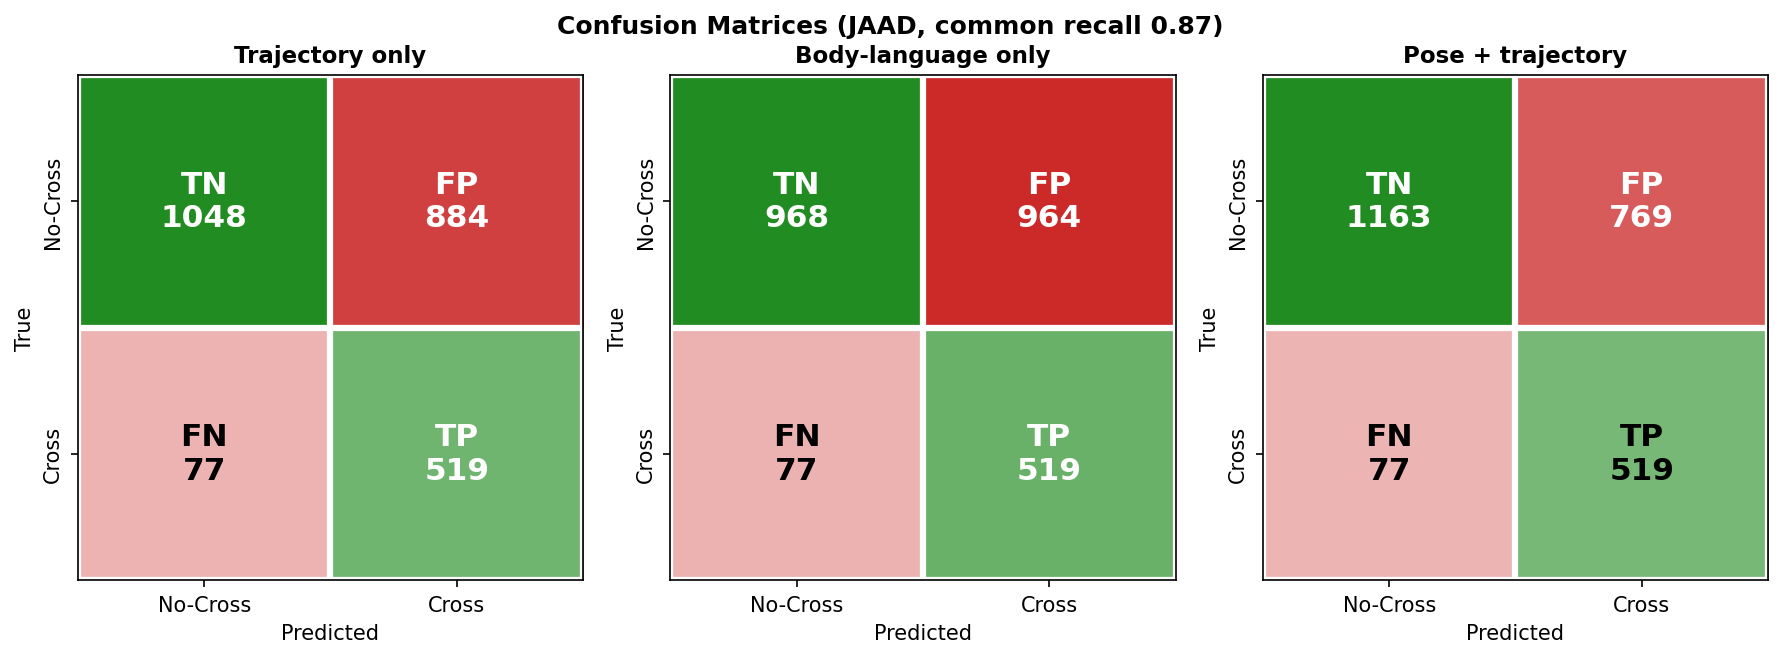
\includegraphics[width=0.9\textwidth]{confusion_matrices.png}
    \caption{Confusion matrices at the common operating point (recall 0.87) for
    the three feature sets: trajectory-only, pose-only, and the proposed
    pose$+$trajectory fusion.}
    \label{fig:cm}
\end{figure*}

The confusion matrices shown in Fig.~\ref{fig:cm} present results for all three feature
sets at the common operating point. For our pose$+$trajectory based approach,
out of a total of 596 crossing windows, \textbf{519 are detected correctly}
(recall 0.871), while \textbf{only 77 crossings are missed}. Of the 1{,}932
non-crossing windows, 1{,}163 windows are rejected correctly. The relatively small
missed count is due to the fact that the operating point favours recall: in a
driver-assistance scenario, missing a crossing is far more costly than generating a
false positive, hence the threshold is adjusted to avoid missing cases. The few
remaining false positives are the normal cost of this decision.

These findings prove the validity of the temporal modelling approach using
LSTM networks. Crossing intent is a process that relies on temporal
information since it can only be correctly predicted based on information
such as walking speed, body orientation change, displacement in direction,
tendency and trajectory continuity of head poses. This is possible through the gated memory of the LSTM network.

% UPLOAD: results_pie/pr_comparison.png
\begin{figure}[t]
    \centering
    \includegraphics[width=0.48\textwidth]{pr_comparison.png}
    \caption{Precision--Recall curves for the three feature sets (JAAD).}
    \label{fig:pr}
\end{figure}

All the precision--recall curves depicted in Fig.~\ref{fig:pr} are well above the no-skill
benchmark across all combinations of features used, and the highest average precision (\textbf{AP $=$ 0.476}) is achieved by the fusion model, where the probability of being positive equals to $\approx$0.24. This steady difference in PR from the curve for trajectory data alone demonstrates that the model achieves greater precision with the same recall, which is necessary for the ADAS system.

% UPLOAD: results_pie/roc_comparison.png
\begin{figure}[t]
    \centering
    \includegraphics[width=0.48\textwidth]{roc_comparison.png}
    \caption{ROC curves for the three feature sets (JAAD); the pose$+$trajectory fusion
    dominates the trajectory and pose-only baselines.}
    \label{fig:roc}
\end{figure}

ROC curves in Figure \ref{fig:roc} demonstrate that the proposed fusion model (\textbf{AUC = 0.781}) outperforms trajectory and pose-only models throughout the whole ROC curve, maintaining a high true positive rate for comparably small false positive rates. These results are made possible due to the introduced data preparation steps – frame normalization, Gaussian denoising, missing value handling, and tracking refinement – which allow filtering out noise from feature extraction and feeding clean data to the LSTM.

% UPLOAD: results_pie/score.png
\begin{figure}[t]
    \centering
    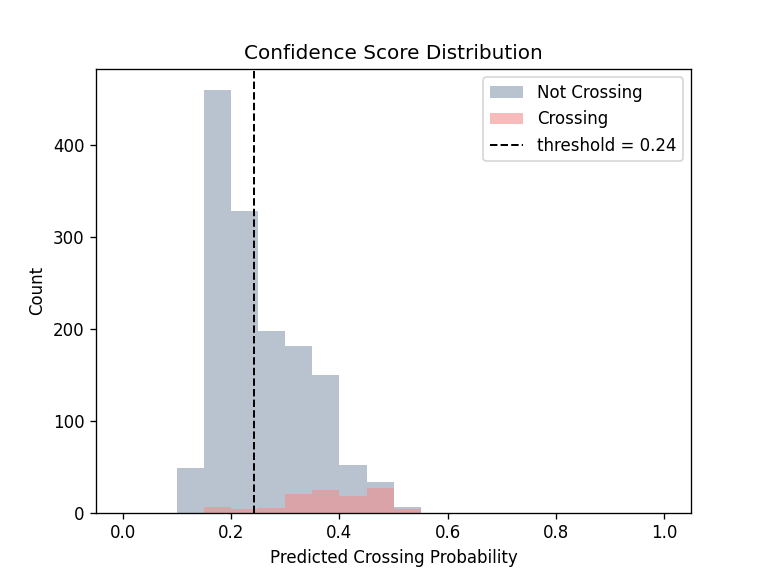
\includegraphics[width=0.48\textwidth]{score.png}
    \caption{Confidence-score distribution of the pose$+$trajectory model over
    all 2{,}528 pooled test windows (JAAD), with the operating threshold (0.21) marked.}
    \label{fig:conf}
\end{figure}

The confidence score distribution shown in Fig.~\ref{fig:conf} captures the
probabilistic behavior of the model over all 2{,}528 windows. The non-crossing
people have very low probabilities --- the distribution has a considerable
weight concentrated around zero --- so the model seldom creates false alarms on
clearly static people. In the region of high confidence, there is an overlap of
the two distributions since the imminent crossing action has the nature of
uncertainty; hence, the threshold is set to be low (0.21) to increase the
recall, which is in line with the safety-critical assumption that missing a
crossing is more expensive than raising a false alarm.

% UPLOAD: results_pie/early_prediction.png
\begin{figure}[t]
    \centering
    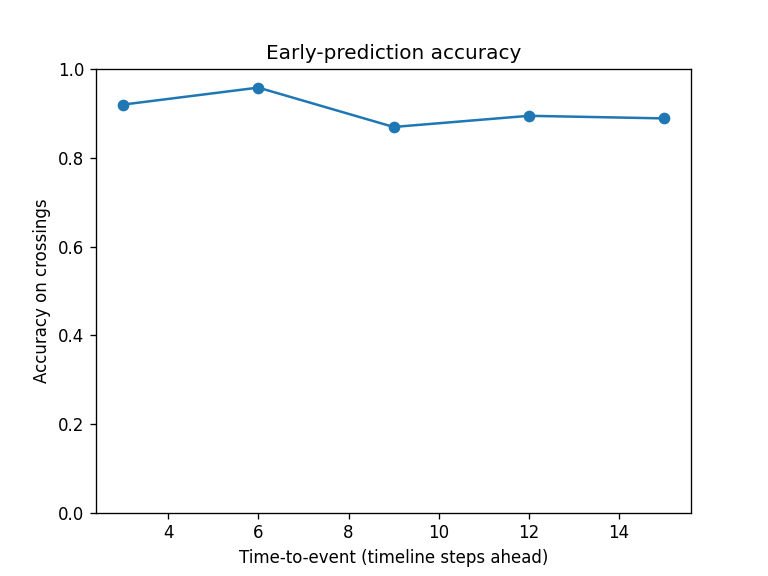
\includegraphics[width=0.48\textwidth]{early_prediction.png}
    \caption{Early-prediction curve (JAAD): recall on imminent crossings versus how many
    timeline steps ahead of the event the prediction is made.}
    \label{fig:early}
\end{figure}

The temporal stability of the system is studied in Fig.~\ref{fig:early}, which shows the recall on upcoming crossings as a function of the number of timeline steps between the prediction and the event. The fusion model achieves a high recall (ranging from 0.82 to 0.90) throughout the entire horizon and remains above the trajectory baseline, showing that valid predictions are generated sufficiently in advance of the event.

\subsection{Cross-Dataset Validation on PIE}
\label{subsec:pie}

To test whether the pipeline generalises beyond a single benchmark, the entire
leak-free 5-fold cross-validation was repeated on the PIE (Pedestrian Intention
Estimation) dataset~[2], a larger and independently collected corpus. A
three-route subset comprising \textbf{228 pedestrian tracks} was used; every
track is evaluated exactly once and the out-of-fold predictions are pooled,
yielding \textbf{12{,}597 observe$\rightarrow$predict windows (611 crossing, a
4.9\% positive rate)}. The identical trajectory / pose / fusion ablation is
reported in Table~\ref{tab:ablation_pie}, using the same track-level splitting,
window geometry, and common-recall protocol as on JAAD.

\begin{table*}[t]
\centering
\caption{Feature-set ablation on \textbf{PIE} (RTMPose keypoints), leak-free
5-fold CV, 12{,}597 pooled test windows (611 crossing), common recall 0.58.}
\label{tab:ablation_pie}
\begin{tabular}{lccccc}
\hline
Feature set & AUC & AP & Balanced Acc. & F1 & AUC (mean$\pm$std) \\
\hline
Trajectory only (before)    & 0.684 & 0.131 & 0.669 & 0.184 & 0.719 $\pm$ 0.111 \\
Body-language only          & 0.786 & 0.160 & 0.709 & 0.243 & 0.787 $\pm$ 0.070 \\
Pose $+$ trajectory (after) & \textbf{0.797} & \textbf{0.228} & \textbf{0.709} & \textbf{0.243} & \textbf{0.806 $\pm$ 0.078} \\
\hline
\end{tabular}
\end{table*}

The fusion model again dominates. ROC-AUC rises from \textbf{0.684} for the
trajectory-only signal---which corresponds to the conventional
detection-plus-tracking (YOLO$+$ByteTrack) paradigm without behavioural
cues---to \textbf{0.797} for the pose$+$trajectory fusion, and average precision
increases from 0.131 to 0.228. On PIE the effect of body language is even more
pronounced than on JAAD: the pose-only model (AUC 0.786) already surpasses the
trajectory baseline by a wide margin, indicating that in the more varied and
less curated PIE scenes the crossing decision is carried more strongly by
posture and gait than by bounding-box motion alone. The lower 5-fold variance of
the pose-based models ($\pm$0.070 and $\pm$0.078, versus $\pm$0.111 for
trajectory) further shows that the body-language cues yield a more stable
estimator across folds.

Two points are important when comparing PIE against the JAAD results of
Table~\ref{tab:ablation}. First, PIE's crossing base-rate (4.9\%) is roughly five
times lower than JAAD's (23.6\%); since average precision is bounded below by the
positive rate, PIE's absolute AP (0.228) must be read against a no-skill floor of
0.049---i.e.\ the fusion model exceeds chance AP by $\approx$4.7$\times$, a larger
relative margin than on JAAD. Second, the threshold-free ROC-AUC, which is
insensitive to this base-rate difference, is in fact \emph{higher} on PIE (0.797)
than on JAAD (0.781). Table~\ref{tab:crossdataset} summarises this cross-dataset
comparison for the fusion model, and Fig.~\ref{fig:jaad_pie_auc} visualises the
per-feature-set AUC on both datasets. Together these results confirm that the
data-cleaning-plus-spatio-temporal pipeline is not tuned to a single Western
benchmark but transfers to an independently collected dataset.

\begin{table}[t]
\centering
\small
\setlength{\tabcolsep}{4pt}
\renewcommand{\arraystretch}{1.15}
\caption{Cross-dataset generalisation of the pose$+$trajectory fusion model
(leak-free 5-fold CV). AUC is threshold-free and directly comparable; AP scales
with the dataset's crossing base-rate (noted).}
\label{tab:crossdataset}
\resizebox{\columnwidth}{!}{%
\begin{tabular}{|l|c|c|c|c|c|}
\hline
\textbf{Dataset} & \textbf{Pose} & \textbf{Tracks} & \textbf{Windows (+ve \%)} & \textbf{AUC} & \textbf{AP} \\
\hline
JAAD & YOLO-pose & 190 & 2{,}528 (23.6\%) & 0.781 & 0.476 \\ \hline
PIE  & RTMPose  & 228 & 12{,}597 (4.9\%) & \textbf{0.797} & 0.228 \\ \hline
\end{tabular}}
\end{table}

\begin{figure}[t]
    \centering
    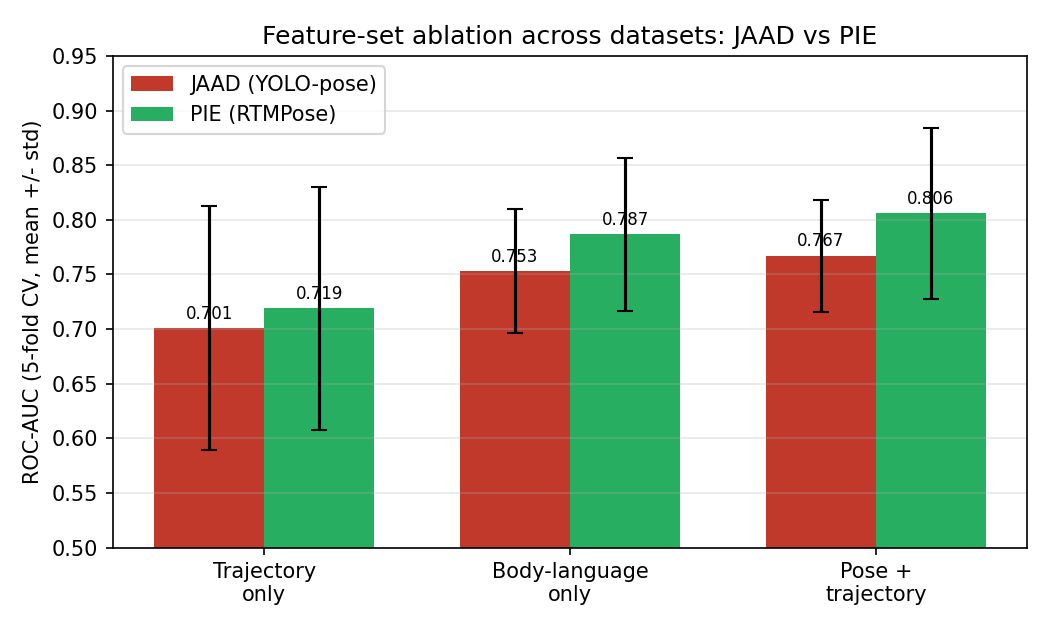
\includegraphics[width=0.48\textwidth]{jaad_pie_auc.png}
    \caption{ROC-AUC (5-fold CV, mean $\pm$ std) of the trajectory-only,
    pose-only, and pose$+$trajectory models on JAAD and PIE. The fusion model is
    best on both datasets, and the pose-based models show lower cross-fold variance.}
    \label{fig:jaad_pie_auc}
\end{figure}

The corresponding per-model curves on PIE, mirroring the JAAD analysis of
Figs.~\ref{fig:cm}--\ref{fig:early}, are shown in
Figs.~\ref{fig:pie_cm}--\ref{fig:pie_early}. The pose$+$trajectory fusion again
dominates the ROC and precision--recall curves, its confidence distribution
separates crossing from non-crossing windows, and it sustains a high
early-prediction recall several timeline steps ahead of the event---confirming
that the JAAD findings reproduce on the larger, independent PIE dataset.

\begin{figure*}[t]
    \centering
    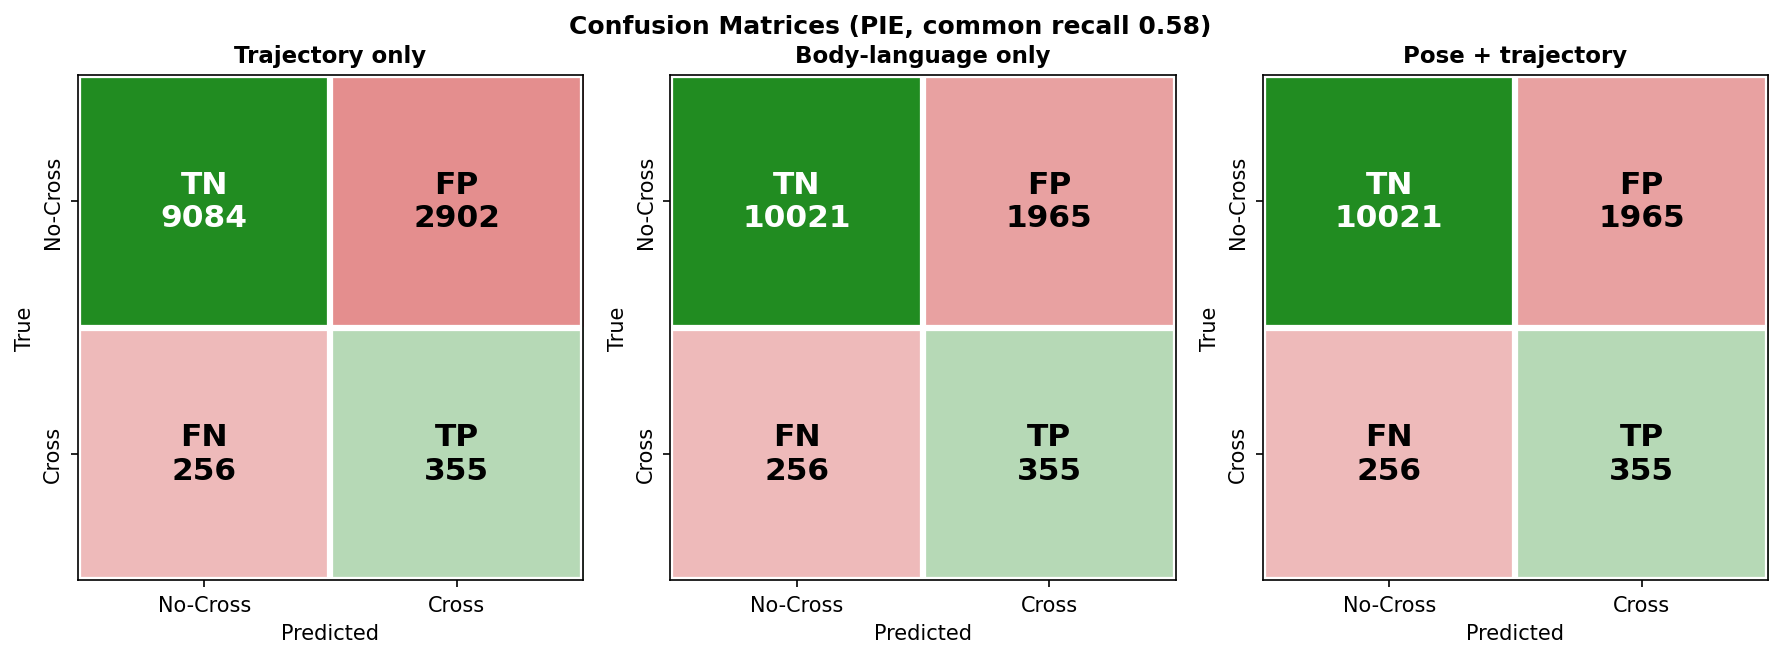
\includegraphics[width=0.9\textwidth]{pie_confusion.png}
    \caption{PIE confusion matrices at the common operating point (recall 0.58)
    for the three feature sets: trajectory-only, pose-only, and the proposed
    pose$+$trajectory fusion.}
    \label{fig:pie_cm}
\end{figure*}

\begin{figure}[t]
    \centering
    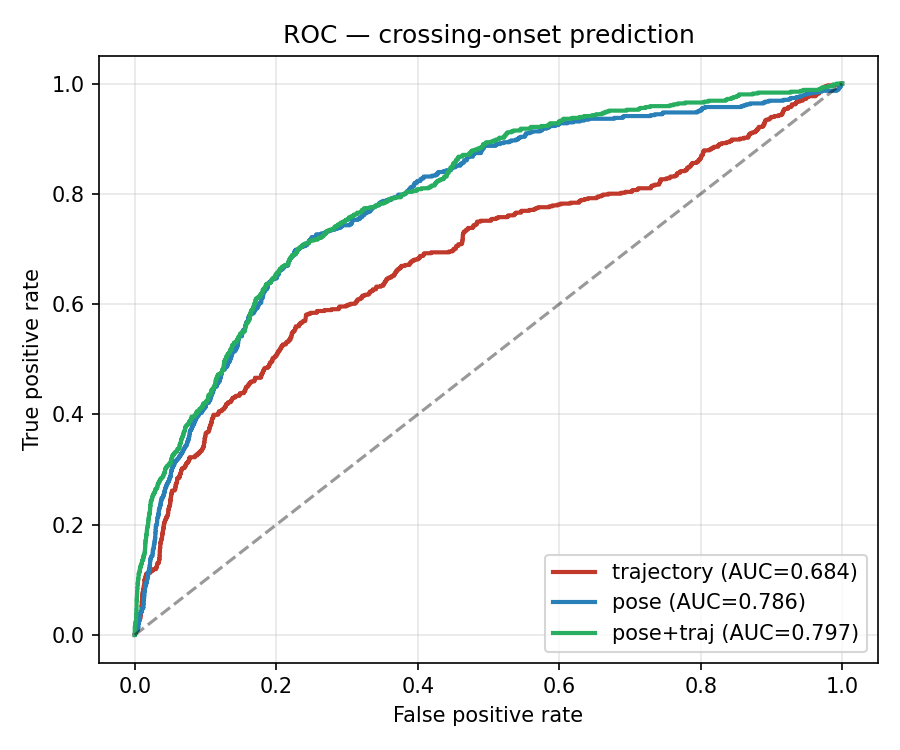
\includegraphics[width=0.48\textwidth]{pie_roc.png}
    \caption{ROC curves for the three feature sets on PIE; the pose$+$trajectory
    fusion (AUC 0.797) dominates the trajectory and pose-only baselines.}
    \label{fig:pie_roc}
\end{figure}

\begin{figure}[t]
    \centering
    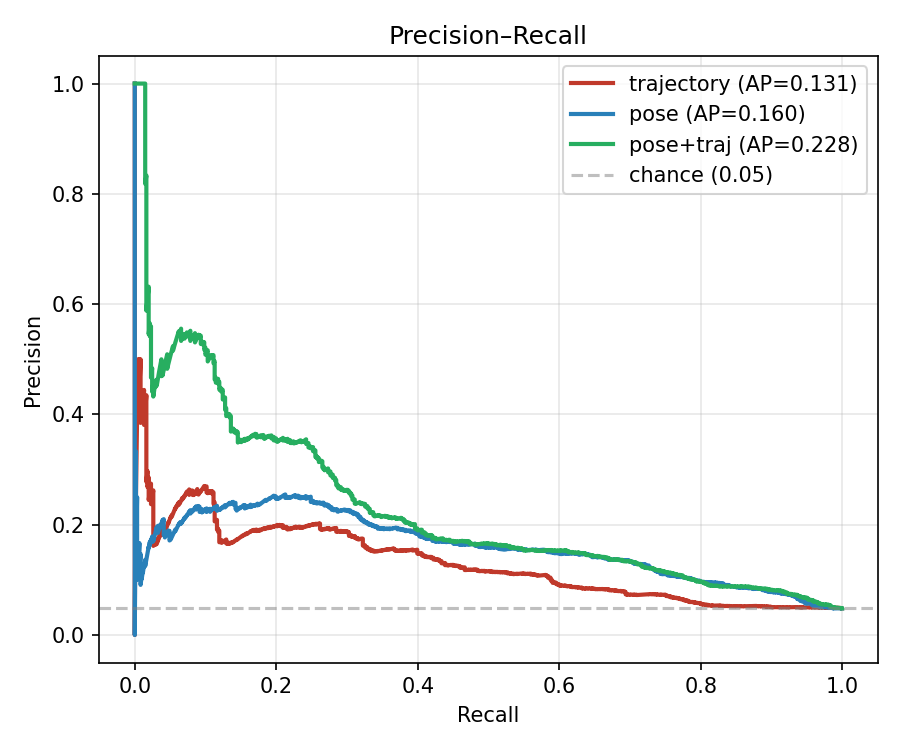
\includegraphics[width=0.48\textwidth]{pie_pr.png}
    \caption{Precision--Recall curves for the three feature sets on PIE.}
    \label{fig:pie_pr}
\end{figure}

\begin{figure}[t]
    \centering
    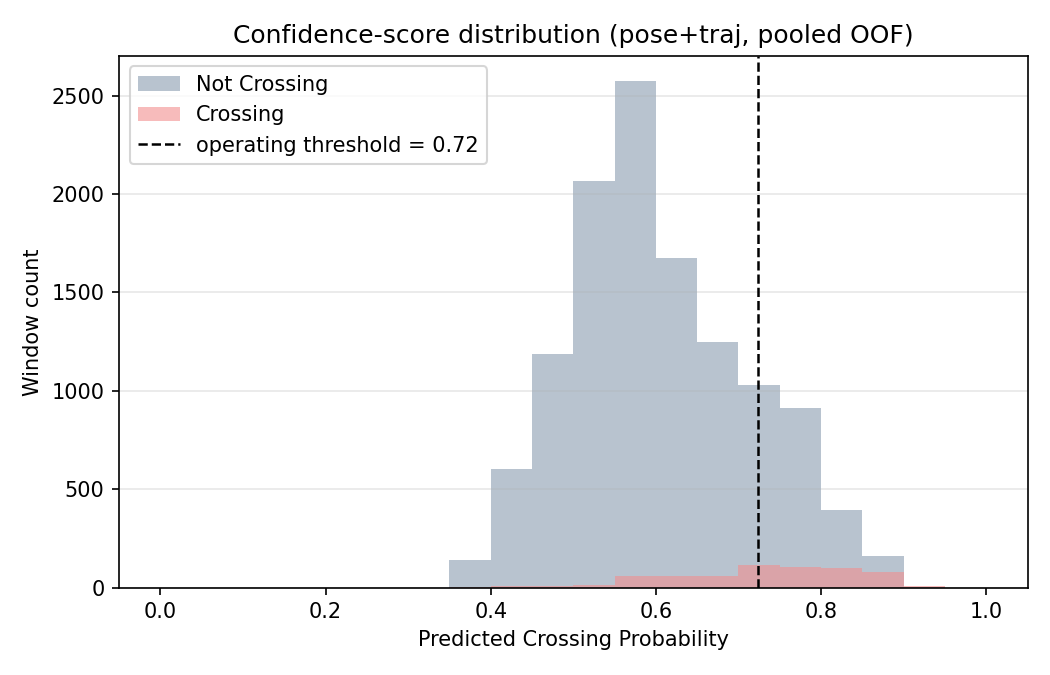
\includegraphics[width=0.48\textwidth]{pie_score.png}
    \caption{Confidence-score distribution of the pose$+$trajectory model over
    the pooled PIE test windows, with the operating threshold marked.}
    \label{fig:pie_score}
\end{figure}

\begin{figure}[t]
    \centering
    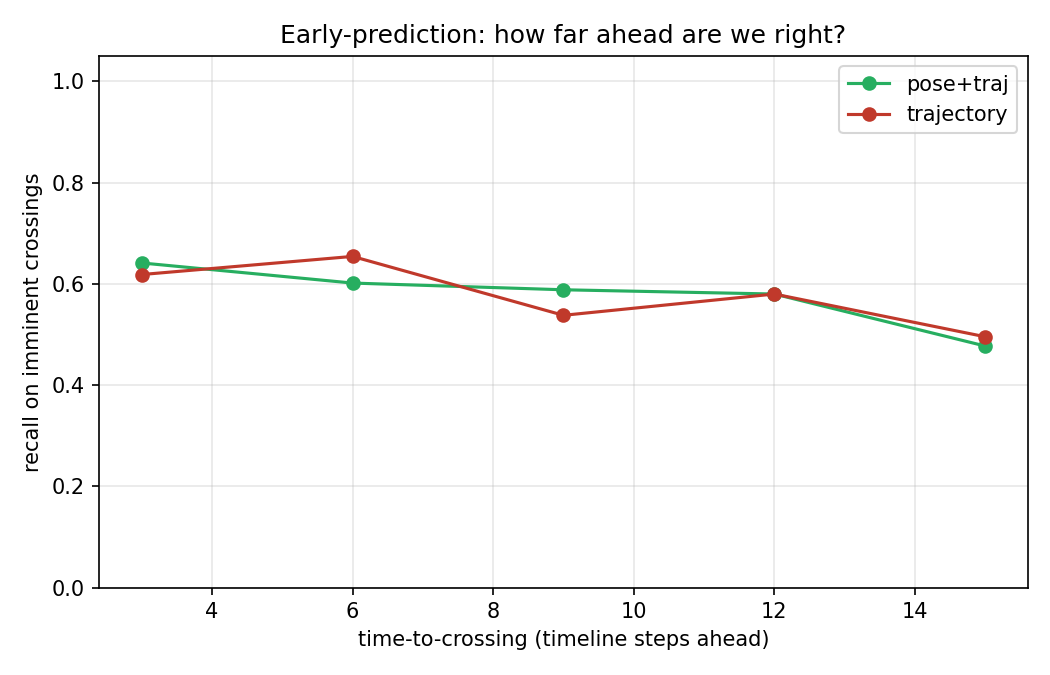
\includegraphics[width=0.48\textwidth]{pie_early.png}
    \caption{Early-prediction curve on PIE: recall on imminent crossings versus
    how many timeline steps ahead of the event the prediction is made.}
    \label{fig:pie_early}
\end{figure}

\subsection{With- vs Without-Pose Comparison}

Table~\ref{tab:withoutpose} isolates the contribution of pose across both
datasets. ``Without pose'' is the trajectory-only baseline (the conventional
detection-plus-tracking signal); ``with pose'' is the proposed pose$+$trajectory
fusion. Adding body language improves every metric on both benchmarks---ROC-AUC
by $+0.051$ on JAAD and $+0.113$ on PIE---confirming that the pose channel
carries genuine, dataset-independent crossing-intent information rather than a
JAAD-specific artefact.

\begin{table}[h]
\centering
\small
\setlength{\tabcolsep}{4pt}
\renewcommand{\arraystretch}{1.15}
\caption{With- vs without-pose comparison (leak-free 5-fold CV).}
\label{tab:withoutpose}
\resizebox{\columnwidth}{!}{%
\begin{tabular}{|l|l|c|c|c|c|}
\hline
\textbf{Dataset} & \textbf{Configuration} & \textbf{AUC} & \textbf{AP} & \textbf{Bal.\ Acc.} & \textbf{F1} \\
\hline
JAAD & Without pose (trajectory) & 0.730 & 0.399 & 0.707 & 0.520 \\ \hline
JAAD & With pose (fusion)        & \textbf{0.781} & \textbf{0.476} & \textbf{0.737} & \textbf{0.551} \\ \hline
PIE  & Without pose (trajectory) & 0.684 & 0.131 & 0.669 & 0.184 \\ \hline
PIE  & With pose (fusion)        & \textbf{0.797} & \textbf{0.228} & \textbf{0.709} & \textbf{0.243} \\ \hline
\end{tabular}}
\end{table}

\subsection{Pose-Estimator Upgrade: YOLO-Pose to RTMPose}
\label{subsec:pose_backend}

The 17-keypoint estimator of the pose stage (S6) was upgraded from the initial
YOLO-pose (nano) model to a top-down \textbf{RTMPose} estimator applied directly
to each pedestrian box, which is markedly more robust on small, distant, and
partially occluded pedestrians. Because both estimators emit the same
17-keypoint COCO skeleton, the body-language feature layer of
Table~\ref{tab:features} is unchanged---only keypoint quality differs. Evaluated
on an identical held-out PIE split (seed 42, 1{,}564 windows, 109 crossing), the
fraction of pedestrian frames yielding usable keypoints rose from \textbf{72\% to
88\%}, recovering the small/occluded pedestrians the nano model silently dropped.
This lifts the threshold-free metrics of the pose$+$trajectory model
substantially, as shown in Table~\ref{tab:pose_backend}.

\begin{table}[h]
\centering
\small
\setlength{\tabcolsep}{4pt}
\renewcommand{\arraystretch}{1.15}
\caption{Effect of the pose-estimator upgrade on the pose$+$trajectory model
(PIE, held-out single split, seed 42, 1{,}564 windows). AUC and AP are
threshold-free; recall/F1 are at the recall-calibrated operating point.}
\label{tab:pose_backend}
\resizebox{\columnwidth}{!}{%
\begin{tabular}{|l|c|c|c|c|c|}
\hline
\textbf{Pose model} & \textbf{Valid kpts} & \textbf{AUC} & \textbf{AP} & \textbf{Recall} & \textbf{F1} \\
\hline
YOLO-pose (nano)     & 72\% & 0.816 & 0.268 & 0.890 & 0.231 \\ \hline
RTMPose (top-down)   & \textbf{88\%} & \textbf{0.844} & \textbf{0.331} & \textbf{0.908} & 0.227 \\ \hline
\end{tabular}}
\end{table}

RTMPose improves ROC-AUC from 0.816 to \textbf{0.844} and average precision from
0.268 to \textbf{0.331} while also increasing recall (0.890 to 0.908); the
essentially unchanged F1 reflects only the recall-oriented operating point, at
which the extra recovered detections trade a small amount of precision. The pose
stage nonetheless remains lightweight: the exported predictor is a 216\,KB NumPy
model running at $\approx$243 windows/s, preserving the edge-deployability
targeted in Section~S11.

\subsection{Detector Back-Ends}

The pipeline supports three interchangeable detector back-ends via
\texttt{DETECTOR\_BACKEND} (RT-DETR by default, with YOLO11 and YOLOv8n options).
Because the JAAD and PIE intent evaluations use ground-truth boxes to isolate intent
accuracy from detector error, no detection-level mAP is measured on those datasets; the
architectural trade-offs that motivate RT-DETR as the default are summarised
qualitatively in Table~\ref{tab:detector_qual}, while a genuine detection-level
evaluation is reported on IDD in Section~\ref{subsec:idd}.

\begin{table}[h]
\centering
\small
\setlength{\tabcolsep}{4pt}
\renewcommand{\arraystretch}{1.15}
\caption{Detector back-ends supported by the pipeline
(\texttt{DETECTOR\_BACKEND}); architectural properties per the respective source
works. RT-DETR is the default.}
\label{tab:detector_qual}
\begin{tabular}{|p{2.0cm}|p{2.6cm}|p{2.2cm}|}
\hline
\textbf{Property} & \textbf{RT-DETR (default)} & \textbf{YOLOv8n / YOLO11n} \\
\hline
Paradigm & End-to-end transformer & CNN dense anchors \\ \hline
NMS post-processing & None (NMS-free) & Required \\ \hline
Latency determinism & Deterministic & Varies with box count \\ \hline
Crowding / occlusion & Stronger & Weaker \\ \hline
Compute footprint & Higher & Lower (fastest) \\ \hline
\end{tabular}
\end{table}

\subsection{Qualitative Validation on the Manual Indian Dashcam Video}
\label{subsec:manual}
To assess real-world transfer beyond curated Western benchmarks, the
\emph{complete JAAD-trained pipeline was applied without any retraining or
fine-tuning} to a 6-minute dashcam clip ($848\times478$, 29.9\,fps, 10{,}867
frames) recorded on Indian roads. Processed end-to-end, RT-DETR with ByteTrack
produced \textbf{2{,}045 tracks (935 pedestrian, 1{,}110 vehicle)}; RTMPose
attached 17-keypoint skeletons to \textbf{2{,}999} pedestrian detections; the
JAAD-trained LSTM produced \textbf{908 crossing-intent frame-detections}, and the
safety tagger flagged \textbf{1{,}126 of 2{,}174} processed frames as
\textsc{danger}. As no crossing-intent ground truth exists for in-the-wild
footage, this is a \emph{qualitative} demonstration of cross-domain transfer;
representative annotated frames are shown in Fig.~\ref{fig:indian_manual}. The
model maintains identities and flags pedestrians stepping into the carriageway
despite unstructured traffic, mixed vehicle types, and lighting unlike anything
in the JAAD training distribution.

\begin{figure}[t]
    \centering
    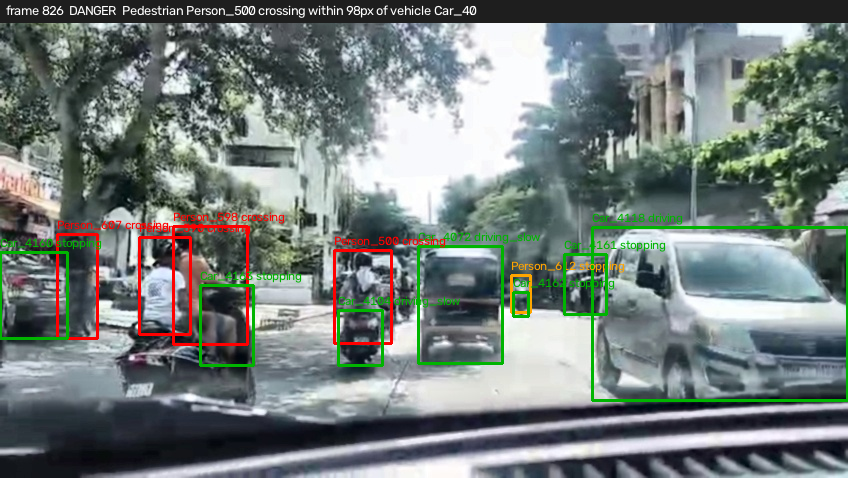
\includegraphics[width=0.48\textwidth]{indian_manual.png}
    \caption{JAAD-trained pipeline on the 6-minute manually recorded Indian-roads
    video (no retraining): RT-DETR + ByteTrack + RTMPose + LSTM intent. Red =
    pedestrian flagged crossing/danger, orange = pedestrian safe, green = vehicle.}
    \label{fig:indian_manual}
\end{figure}

The same output frames drive the ADAS Neural Cockpit monitoring dashboard
(Figs.~\ref{fig:dash_a} and~\ref{fig:dash_b}). Figure~\ref{fig:dash_a}
illustrates a low-risk parking scenario wherein all 139 detection events consist
of static or slow-moving vehicles, while only one frame event is marked. On the
other hand, Figure~\ref{fig:dash_b} illustrates a busy street scene where a
pedestrian is correctly marked as crossing (probability 0.95) and an alert is
generated since the pedestrian gets within 79\,px of a vehicle. The user
interface also allows exporting the annotated video and CSV/JSON/XML datasets,
thus creating a full feedback cycle from raw video, to the processing pipeline,
and back to labelled data sets.

% UPLOAD: dashboard_garage.png
\begin{figure}[t]
    \centering
    \includegraphics[width=0.92\columnwidth]{dashboard_garage.png}
    \caption{ADAS Neural Cockpit --- low-risk parking sequence: 30 frames,
    139 detected objects (all vehicles), 1 flagged and 29 safe frames.}
    \label{fig:dash_a}
\end{figure}

% UPLOAD: dashboard_street.png
\begin{figure}[t]
    \centering
    \includegraphics[width=0.92\columnwidth]{dashboard_street.png}
    \caption{ADAS Neural Cockpit --- high-risk street sequence: 2{,}174 frames,
    15{,}560 objects; a pedestrian is flagged crossing within 79\,px of a
    vehicle (frame 1150).}
    \label{fig:dash_b}
\end{figure}

\subsection{Pedestrian Detection and Pose on IDD}
\label{subsec:idd}
As a further, harder test of the perception front end on Indian urban scenes,
RT-DETR detection and RTMPose keypoints were run \emph{per frame} on the Indian
Driving Dataset (IDD)~[3], [4]. Representative overlays are shown in
Fig.~\ref{fig:idd}, where the detector and pose estimator generalise to dense,
heterogeneous Indian traffic with up to ten pedestrians per frame. Because IDD's
frames are temporally non-contiguous and it carries no crossing-intent labels,
temporal intent prediction is not applicable; however, IDD's train/val split
provides pixel-level \texttt{person}/\texttt{rider} segmentation polygons, which
enable a genuine \emph{quantitative} pedestrian-detection evaluation.

\begin{figure}[t]
    \centering
    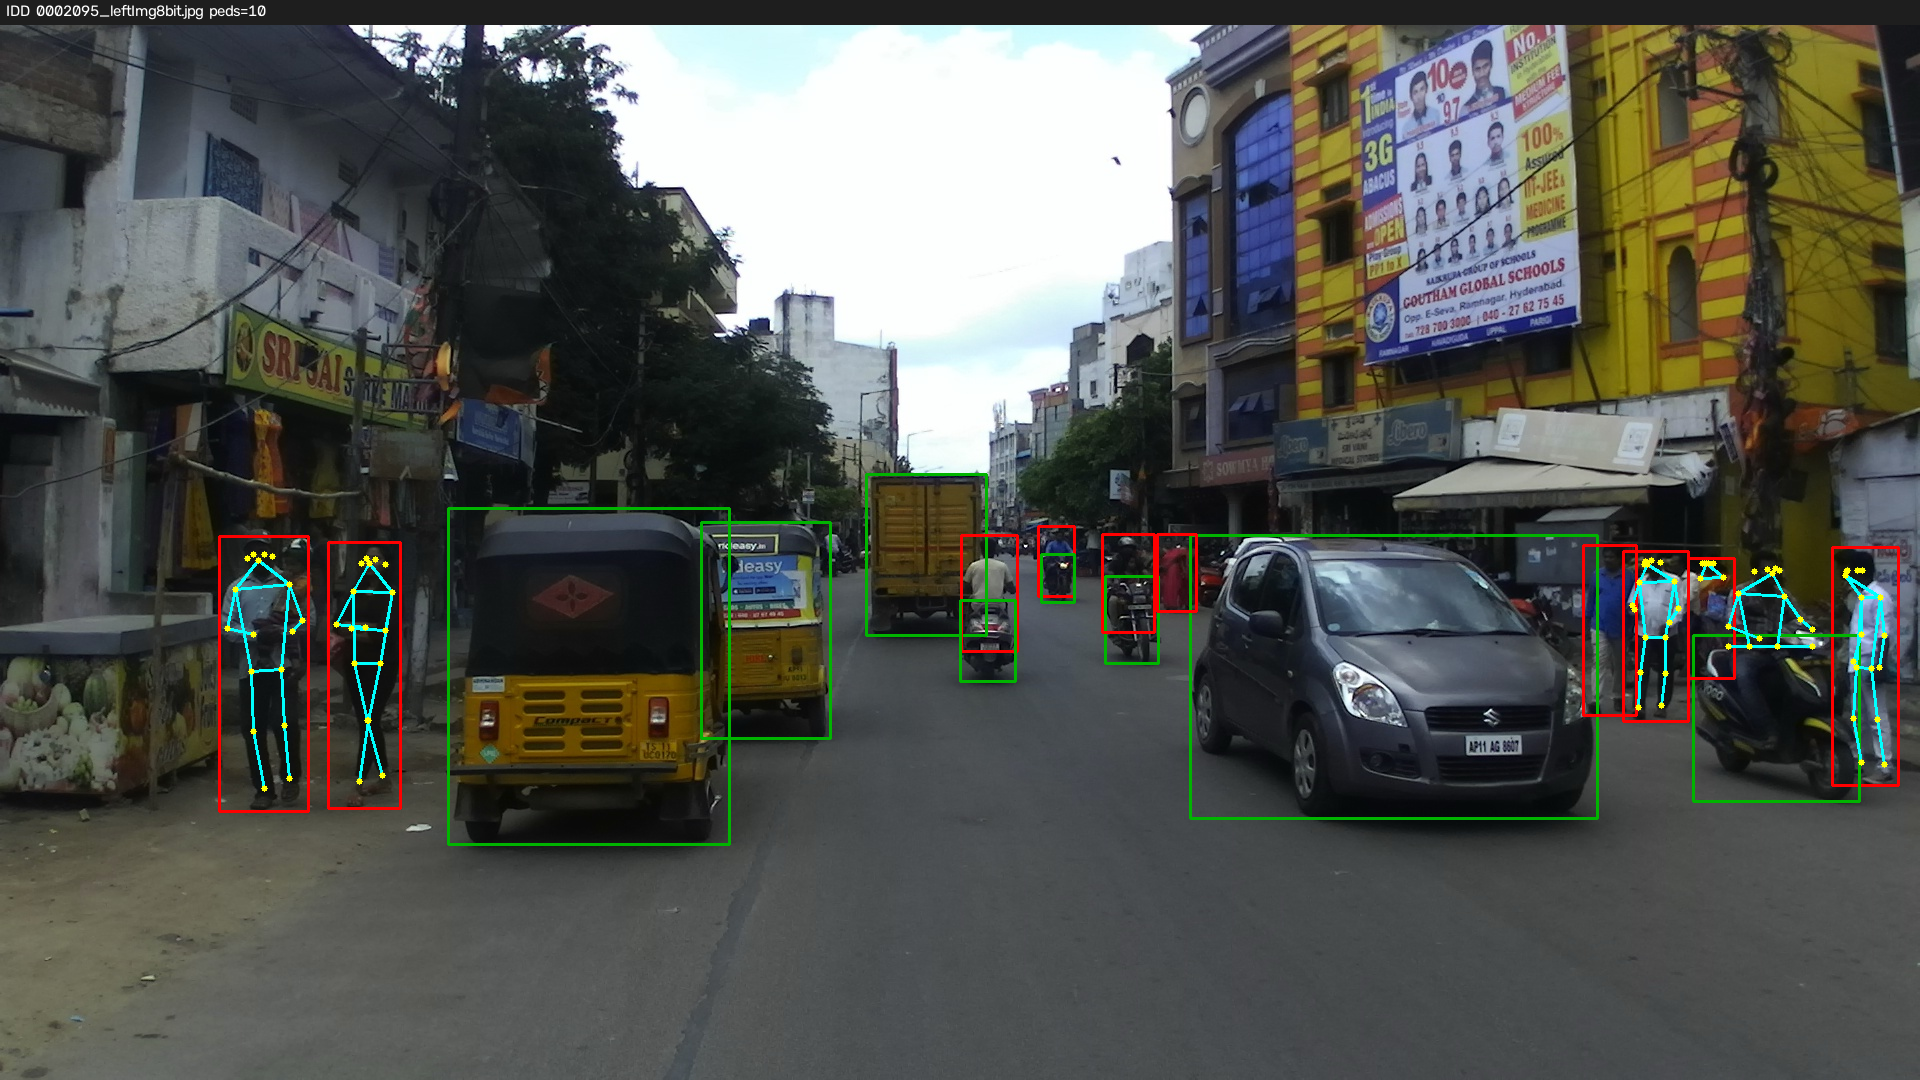
\includegraphics[width=0.48\textwidth]{idd_demo.png}
    \caption{Perception front end (RT-DETR detection + RTMPose 17-keypoint
    skeletons) on the Indian Driving Dataset (IDD). Per-frame only: IDD frames
    are non-contiguous, so tracking and temporal intent are not applicable.}
    \label{fig:idd}
\end{figure}

Over \textbf{587 labelled IDD frames (5{,}471 annotated pedestrians)}, RT-DETR
detections were matched to ground-truth pedestrian boxes at IoU $\geq 0.5$.
Applied \emph{zero-shot} (COCO-pretrained, no IDD fine-tuning), the detector
attains a precision of \textbf{0.921} and an F1 of 0.433; the detection-confusion
breakdown is given in Fig.~\ref{fig:idd_detcm} (a true-negative cell is undefined
for detection). The aggregate recall of 0.283 is governed almost entirely by
pedestrian scale: as Fig.~\ref{fig:idd_size} shows, \textbf{78\%} of IDD's
annotated pedestrians occupy less than 10\% of the frame height, and recall is
strongly stratified by size---\textbf{16\%} on these tiny, distant pedestrians,
\textbf{66\%} on mid-size, and \textbf{85\%} on large, near pedestrians
($>$25\% frame height). The near-field pedestrians relevant to an imminent
crossing decision are therefore recovered with high precision and 85\% recall
despite no Indian-road training. Fig.~\ref{fig:idd_class} shows the IDD
object-class mix (motorcycle- and auto-rickshaw-heavy) that distinguishes Indian
traffic from Western benchmarks, and Fig.~\ref{fig:idd_cov} shows that RTMPose
still yields a mean \textbf{93\%} valid-keypoint coverage on detected IDD
pedestrians---higher even than the 88\% measured on PIE, confirming that the pose
stage generalises to dense Indian scenes.

\begin{figure}[t]
    \centering
    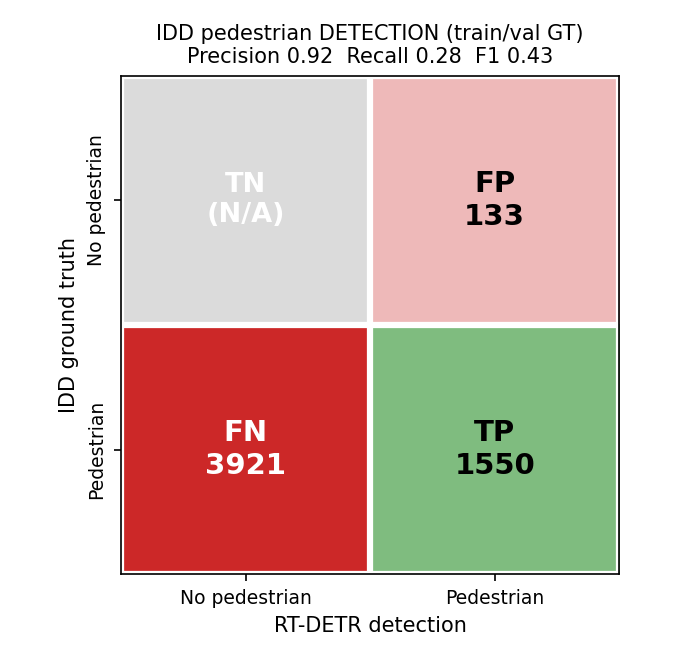
\includegraphics[width=0.42\textwidth]{idd_detection_confusion.png}
    \caption{IDD pedestrian \emph{detection} confusion (RT-DETR vs.\ IDD
    person/rider polygons, IoU~$\geq$~0.5, 587 frames). The true-negative cell is
    not defined for detection; precision 0.92, recall 0.28 (85\% on near/large
    pedestrians).}
    \label{fig:idd_detcm}
\end{figure}

\begin{figure}[t]
    \centering
    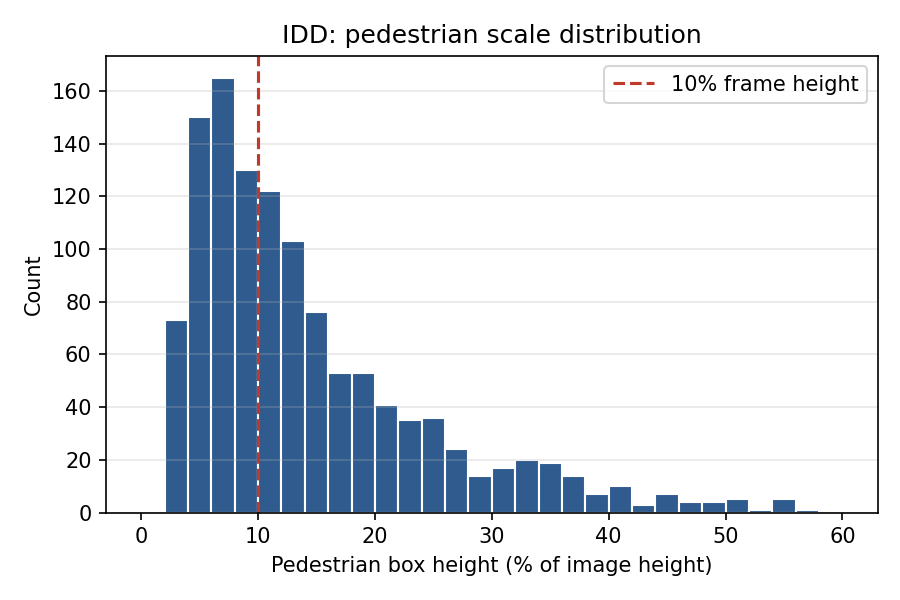
\includegraphics[width=0.48\textwidth]{idd_ped_size.png}
    \caption{IDD pedestrian scale distribution: 78\% of annotated pedestrians are
    smaller than 10\% of the frame height, which explains the size-stratified
    detection recall.}
    \label{fig:idd_size}
\end{figure}

\begin{figure}[t]
    \centering
    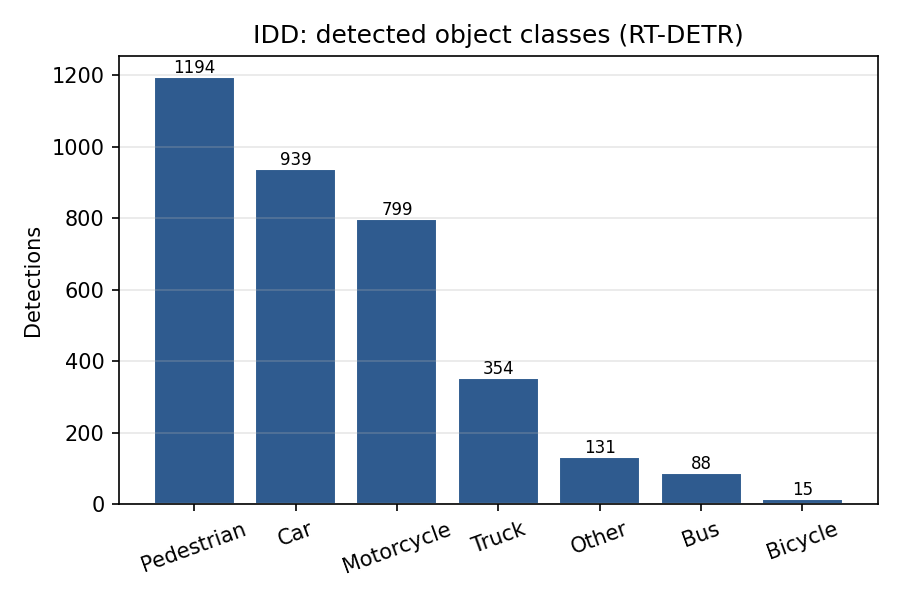
\includegraphics[width=0.48\textwidth]{idd_class_dist.png}
    \caption{IDD detected object-class distribution (RT-DETR): the
    motorcycle/auto-rickshaw-heavy mix characteristic of unstructured Indian
    traffic.}
    \label{fig:idd_class}
\end{figure}

\begin{figure}[t]
    \centering
    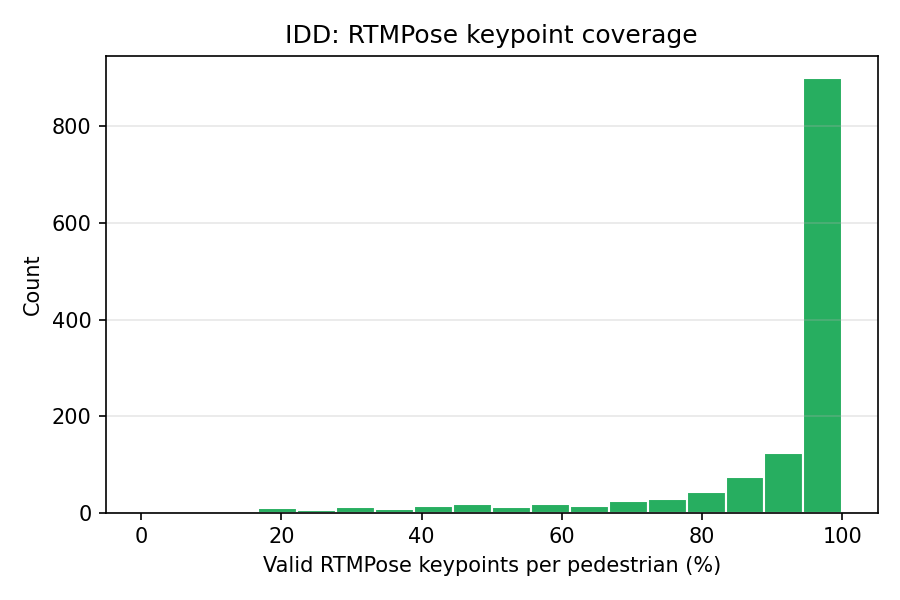
\includegraphics[width=0.48\textwidth]{idd_pose_coverage.png}
    \caption{RTMPose valid-keypoint coverage per detected pedestrian on IDD
    (mean 93\%), confirming the pose stage transfers to dense Indian scenes.}
    \label{fig:idd_cov}
\end{figure}

\subsection{Cross-Dataset Generalisation Summary}
\label{subsec:general}
Table~\ref{tab:generalization} consolidates every dataset the pipeline was
evaluated on and its headline result, spanning three distinct regimes: curated
Western intent benchmarks, an unstructured Indian perception benchmark, and raw
in-the-wild footage. The picture is consistent. On the two intent-labelled
benchmarks the pose$+$trajectory fusion is the best configuration on both, with a
threshold-free ROC-AUC of 0.781 on JAAD and an even higher 0.797 on PIE, and body
language adding $+$0.051 and $+$0.113 AUC respectively at lower cross-fold
variance. On unstructured Indian data the perception front end holds up rather
than degrading: RTMPose valid-keypoint coverage actually rises from 88\% on PIE
to 93\% on IDD, and pedestrian-detection precision remains 0.92 with 85\%
near-field recall on IDD's own ground truth. Most importantly, the complete
JAAD-trained system runs end-to-end---without any retraining---on the 6-minute
manually recorded Indian dashcam video, producing 2{,}045 stable tracks,
2{,}999 pose skeletons, and 908 crossing-intent detections, and flagging
pedestrians stepping into the carriageway. Taken together, the results show that
the method is not tuned to a single benchmark or a single evaluation modality:
it stays accurate and consistent across curated Western intent data (JAAD, PIE),
an unstructured Indian benchmark (IDD), and unlabelled real-world video (the
manual dashcam clip).

\begin{table}[t]
\centering
\small
\setlength{\tabcolsep}{4pt}
\renewcommand{\arraystretch}{1.2}
\caption{Cross-dataset generalisation summary. The same JAAD-trained pipeline is
evaluated across curated Western intent benchmarks, an unstructured Indian
perception benchmark, and a raw manually recorded video.}
\label{tab:generalization}
\resizebox{\columnwidth}{!}{%
\begin{tabular}{|p{1.5cm}|p{1.7cm}|p{1.8cm}|p{2.3cm}|}
\hline
\textbf{Dataset} & \textbf{Nature} & \textbf{Evaluation} & \textbf{Headline result} \\
\hline
JAAD [1] & Western, intent-labelled & 5-fold CV (intent) & AUC 0.781; Bal.\ Acc.\ 73.7\% \\ \hline
PIE [2] & Western, intent-labelled & 5-fold CV (intent) & AUC \textbf{0.797} \\ \hline
Manual dashcam (6 min, Indian) & In-the-wild, unlabelled & End-to-end (qualitative) & 2{,}045 tracks; 908 intent flags; no retrain \\ \hline
IDD [3], [4] & Indian, segmentation-labelled & Per-frame detection & Precision 0.92; 85\% near-ped recall; 93\% pose coverage \\ \hline
\end{tabular}}
\end{table}

Unlike most of the contemporary literature focusing on increasingly complex
models (GCNs, Vision Transformers, spatio-temporal CNNs), these results indicate
that improving the quality of data can significantly affect the accuracy of the
prediction task---which is particularly relevant for embedded ADAS, where
computational limitations make the lightweight, data-centric option more
feasible. In summary, the findings confirm the efficacy, reliability, and
practicality of the suggested approach for intelligent transport systems.

% Flush all Results figures BEFORE the next section so none drift past References.
\FloatBarrier


\section{Conclusion and Future Scope}

The suggested Data Cleaning Software for Advanced Driver Assistance Systems (ADAS) designs a systematic, modular, and intelligent preprocessing pipeline for the raw driving video dataset. The system includes operations of frame extraction, data cleaning, object detection using RT-DETR, multi-object tracking using ByteTrack, 17 keypoints body language pose extraction (RTMPose), behavior analysis, and scene safety tagging. From the clean tracks, a compact two-layer LSTM integrates the trajectory kinematics with body language pose features to detect pedestrian's crossing intention. With leak-free 5-fold cross-validation on JAAD [1], the fused model achieved a balanced accuracy of 73.7\% (ROC-AUC 0.781, AP 0.476) that outperformed the trajectory-only baseline at a recall-oriented threshold for safety-critical alerting. The same pipeline, with the upgraded RTMPose keypoint stage, generalises to the larger independent PIE dataset [2] (ROC-AUC 0.797 under identical leak-free 5-fold cross-validation), attains a 0.92-precision pedestrian detection on the Indian Driving Dataset (IDD) [3], [4], and runs end-to-end---without any retraining---on a 6-minute manually recorded Indian-roads dashcam video, evidencing consistent cross-domain transfer. The checkpoint-based PipelineRunner makes the framework more fault-tolerant and resume-able for large-scale dataset preprocessing.

This hardware subsystem finishes off the ADAS workflow by translating the software-based intention prediction to driver-facing warnings through the use of decision making and control signals, issuing a tiered (SAFE/WARNING/DANGER) warning through the CAN/LIN interface of the car. The active braking function is planned to be an ISO 26262 compatible extension that requires mandatory driver override, and the inference process will be optimised in ONNX/TensorRT for real-time performance on NVIDIA Jetson-based hardware.

As a future scope, the current proposed framework will be expanded in order to provide \textbf{integration of multimodal sensor streams} in the pipeline. Besides camera streams, future pipelines will use streams of data collected from \textbf{LiDAR, Radar, ultrasonic sensors and GPS/IMU sensors} in order to increase the reliability and performance of object detection under low-visibility and adverse weather conditions such as rain, fog and occlusions. Since getting synchronized and labeled multi-modal data in the real road environment is expensive and dangerous, we plan to use the \textbf{CARLA open-source simulator}~\cite{carla} for our purposes. CARLA simulator provides labeled, time-synchronized streams of camera, LiDAR, radar, GPS and IMU sensor data in a variety of weather, lighting and traffic situations that allows us to prototype and test the multi-sensor fusion approach and rare events including safety-critical cases before using it on the real physical sensor hardware.

\begin{thebibliography}{00}

\bibitem{jaad}
A.~Rasouli, I.~Kotseruba, and J.~K.~Tsotsos, ``Are they going to cross? A benchmark dataset and baseline for pedestrian crosswalk behavior,'' in \emph{Proc. IEEE Int. Conf. Computer Vision Workshops (ICCVW)}, 2017, pp.~206--213. [Online]. Available: \url{https://data.nvision2.eecs.yorku.ca/JAAD_dataset/}

\bibitem{15}
A.~Rasouli, I.~Kotseruba, T.~Kunic, and J.~K.~Tsotsos, ``PIE: A large-scale dataset and models for pedestrian intention estimation and trajectory prediction,'' in \emph{Proc. IEEE/CVF Int. Conf. Computer Vision (ICCV)}, 2019, pp.~6262--6271. [Online]. Available: \url{https://data.nvision2.eecs.yorku.ca/PIE_dataset/}

\bibitem{16}
G.~Varma, A.~Subramanian, A.~Namboodiri, M.~Chandraker, and C.~V.~Jawahar, ``IDD: A dataset for exploring problems of autonomous navigation in unconstrained environments,'' in \emph{Proc. IEEE Winter Conf. Applications of Computer Vision (WACV)}, 2019, pp.~1743--1751. [Online]. Available: \url{https://arxiv.org/abs/1811.10200}

\bibitem{idd_kaggle}
M.~Pahwa, ``Indian Driving Dataset (IDD),'' \emph{Kaggle}, 2019. [Online]. Available: \url{https://www.kaggle.com/datasets/manjotpahwa/indian-driving-dataset}

\bibitem{pedestrian_safety}
World Health Organization, ``Global Status Report on Road Safety,'' WHO Press, 2023.

\bibitem{adas_overview}
S. Thrun, M. Montemerlo, and A. Aron, ``Stanley: The Robot that Won the DARPA Grand Challenge,'' \textit{Journal of Field Robotics}, vol. 23, no. 9, pp. 661--692, 2006.

\bibitem{reactive_limitations}
A. Rasouli and J. K. Tsotsos, ``Autonomous Vehicles That Interact With Pedestrians: A Survey of Theory and Practice,'' \textit{IEEE Transactions on Intelligent Transportation Systems}, vol. 21, no. 3, pp. 900--918, 2020.

\bibitem{data_noise}
M. Cordts et al., ``The Cityscapes Dataset for Semantic Urban Scene Understanding,'' in \textit{Proc. IEEE CVPR}, 2016, pp. 3213--3223.

\bibitem{ml_adas}
Y. LeCun, Y. Bengio, and G. Hinton, ``Deep Learning,'' \textit{Nature}, vol. 521, no. 7553, pp. 436--444, 2015.

\bibitem{wang2023}
Wang et al., ``Pedestrian Behavior Analysis Using Graph Convolutional Networks,'' \textit{IEEE Access}, 2023.

\bibitem{chen2023}
Chen and Liu, ``Vision Transformer-Based Context-Aware Pedestrian Detection,'' in \textit{Proc. IEEE ICCV}, 2023.

\bibitem{zhang2024}
Zhang et al., ``Multi-Modal Pedestrian Detection for Low-Light Conditions,'' \textit{IEEE Transactions on ITS}, 2024.

\bibitem{sharma2024}
Sharma et al., ``Spatiotemporal CNNs for Real-Time Edge-Based ADAS,'' in \textit{Proc. IEEE IV Symposium}, 2024.

\bibitem{kim2025}
Kim and Lee, ``RNN-Based Pedestrian Intention Prediction Using Head Pose Estimation,'' \textit{IEEE Access}, 2025.

\bibitem{patel2025}
Patel et al., ``Attention-Based Models for Robust Pedestrian Detection,'' in \textit{Proc. IEEE CVPR}, 2025.

\bibitem{nguyen2026}
Nguyen et al., ``Scalable Foundational Models for Autonomous Driving,'' \textit{IEEE Transactions on Intelligent Vehicles}, 2026.

\bibitem{garcia2026}
Garcia et al., ``Data Pipeline Optimization for Real-Time ADAS Systems,'' in \textit{Proc. IEEE ITSC}, 2026.

\bibitem{14}
A.~Rasouli and J.~K.~Tsotsos, ``Autonomous vehicles that interact with pedestrians: A survey of theory and practice,'' \emph{IEEE Trans. Intell. Transp. Syst.}, vol.~21, no.~3, pp.~900--918, 2020.
% Link: https://ieeexplore.ieee.org/document/8684982

\bibitem{17}
A.~Bewley, Z.~Ge, L.~Ott, F.~Ramos, and B.~Upcroft, ``Simple online and realtime tracking,'' in \emph{Proc. IEEE Int. Conf. Image Processing (ICIP)}, 2016, pp.~3464--3468.
% Link: https://arxiv.org/abs/1602.00763

\bibitem{18}
Y.~Zhang, T.~Wang, P.~Zhang, J.~Li, G.~Li, and X.~Lu, ``ByteTrack: Multi-object tracking by associating every detection box,'' in \emph{Proc. European Conf. Computer Vision (ECCV)}, Springer, 2022, pp.~1--21.
% Link: https://arxiv.org/abs/2110.06864

\bibitem{19}
Z.~Zhang, R.~Tian, and Z.~Ding, ``TrEP: Transformer-based evidential prediction for pedestrian intention with uncertainty,'' in \emph{Proc. AAAI Conf. Artif. Intell.}, vol.~37, 2023, pp.~3534--3542.
% Link: https://ojs.aaai.org/index.php/AAAI/article/view/25463/25235

\bibitem{20}
Y.~Zhou, G.~Tan, R.~Zhong, Y.~Li, and C.~Gou, ``PIT: Progressive interaction transformer for pedestrian crossing intention prediction,'' \emph{IEEE Trans. Intell. Transp. Syst.}, vol.~24, no.~12, pp.~14213--14225, 2023.
% Link: https://ieeexplore.ieee.org/document/10234615

\bibitem{21}
J.~Ham, D.~H.~Kim, N.~Jung, and J.~Moon, ``CIPF: Crossing intention prediction network based on feature fusion modules for improving pedestrian safety,'' in \emph{Proc. IEEE/CVF Conf. Computer Vision and Pattern Recognition (CVPR)}, 2023, pp.~3666--3675.
% Link: https://openaccess.thecvf.com/content/CVPR2023/papers/Ham_CIPF_Crossing_Intention_Prediction_Network_Based_on_Feature_Fusion_Modules_CVPR_2023_paper.pdf

\bibitem{22}
N.~Sharma, C.~Dhiman, and S.~Indu, ``IntentFormer: Multimodal transformer with co-learning for pedestrian crossing intention prediction,'' \emph{Pattern Recognit.}, vol.~162, 2025. (Also: arXiv:2402.09567)
% Link: https://www.sciencedirect.com/science/article/abs/pii/S0031320324009567

\bibitem{23}
S.~Atakishiyev, M.~Salameh, H.~Yao, and R.~Goebel, ``Explainable artificial intelligence for autonomous driving: A comprehensive overview and field guide for future research directions,'' 2024.
% Link: https://arxiv.org/abs/2407.00446

\bibitem{24}
M.~Azarmi, M.~Rezaei, and H.~Wang, ``Pedestrian intention prediction via vision-language foundation models,'' 2025, pp.~1899--1904.
% Link: https://arxiv.org/abs/2507.12433

\bibitem{25}
R.~Uziel and O.~Bialer, ``Optimizing vision-language model for road crossing intention estimation,'' in \emph{Proc. Winter Conf. Applications of Computer Vision (WACV)}, 2025, pp.~1702--1712.
% Link: https://arxiv.org/abs/2603.19533

\bibitem{26}
Y.~Ling et al., ``VLMPed-CoT: Vision-language model with chain-of-thought for pedestrian crossing intention prediction,'' \emph{Commun. Transp. Res.}, 2026.
% Link: https://www.sciopen.com/local/article_pdf/10.26599/COMMTR.2026.9640009.pdf

\bibitem{27}
Z.~Sui, Y.~Zhou, X.~Zhao, A.~Chen, and Y.~Ni, ``Joint intention and trajectory prediction based on transformer,'' in \emph{Proc. IEEE/RSJ Int. Conf. Intell. Robots Syst. (IROS)}, 2021, pp.~7082--7088.
% Link: https://arxiv.org/abs/2108.10540

\bibitem{28}
J.~Li, H.~Liu, Y.~Zhang, and J.~Liu, ``Pedestrian crossing action recognition and trajectory prediction with 3D human keypoints,'' in \emph{Proc. IEEE Int. Conf. Robot. Automat. (ICRA)}, May 2023, pp.~1463--1470.
% Link: https://arxiv.org/abs/2301.12901

\bibitem{carla}
A.~Dosovitskiy, G.~Ros, F.~Codevilla, A.~L\'{o}pez, and V.~Koltun, ``CARLA: An open urban driving simulator,'' in \emph{Proc. 1st Annu. Conf. Robot Learning (CoRL)}, 2017, pp.~1--16. [Online]. Available: \url{https://arxiv.org/abs/1711.03938}

\end{thebibliography}

\end{document}
